% Revamped manuscript for ARC project.
% Self-contained LaTeX: no external figure-data files are required.
% Compile twice with pdflatex: pdflatex arc_revamped.tex
\documentclass[11pt]{article}

\usepackage[margin=0.8in]{geometry}
\usepackage[T1]{fontenc}
\usepackage{lmodern}
\usepackage{microtype}
\usepackage{amsmath,amssymb,mathtools}
\usepackage{graphicx}
\usepackage{booktabs,longtable,tabularx,array,multirow}
\usepackage{enumitem}
\usepackage{setspace}
\usepackage{xcolor}
\usepackage{tikz}
\usetikzlibrary{arrows.meta,positioning,shapes.geometric,fit,calc,backgrounds}
\usepackage{pgfplots}
\usepackage{caption}
\usepackage{subcaption}
\usepackage[colorlinks=true,linkcolor=blue!50!black,citecolor=blue!50!black,urlcolor=blue!55!black]{hyperref}
\usepackage[nameinlink,noabbrev]{cleveref}
\usepackage{algorithm}
\usepackage{algpseudocode}
\captionsetup[algorithm]{font=small}
\pgfplotsset{compat=1.18}
\setstretch{1.02}
\setlength{\parindent}{1.2em}
\setlength{\parskip}{0.12em}
\setlist[enumerate]{leftmargin=*,itemsep=0.25em,topsep=0.3em}
\setlist[itemize]{leftmargin=*,itemsep=0.2em,topsep=0.3em}
\setlength{\textfloatsep}{10pt plus 2pt minus 2pt}
\setlength{\intextsep}{8pt plus 2pt minus 2pt}
\renewcommand{\arraystretch}{1.05}

\definecolor{attncol}{HTML}{1769AA}
\definecolor{mlpcol}{HTML}{C55342}
\definecolor{isiccol}{HTML}{26856B}
\definecolor{lightblue}{HTML}{E8F1FA}
\definecolor{lightorange}{HTML}{F9ECE7}
\definecolor{lightgreen}{HTML}{E6F3EE}
\definecolor{midgray}{HTML}{636B74}
\newcommand{\pp}{\,\text{pp}}
\newcommand{\pct}[1]{#1\%}
\newcommand{\meanSD}[2]{#1 $\pm$ #2}
\newcommand{\method}[1]{\texttt{#1}}
\newcolumntype{Y}{>{\raggedright\arraybackslash}X}
\newcolumntype{P}[1]{>{\raggedright\arraybackslash}p{#1}}

\title{Where You Adapt Beats What You Adapt\\[0.25em]
\large A Controlled Study of Adaptation Depth in Cross-Domain Few-Shot Vision}
\author{Ariet Jha}
\date{October 2026}

\begin{document}
\maketitle

\begin{abstract}
Parameter-efficient fine-tuning is usually organised around \emph{which} family of
parameters is updated: attention projections, feed-forward layers, normalisation
parameters, or a low-rank factor. This paper studies a complementary axis,
\emph{where} an otherwise fixed adaptation is applied. Using a supervised
ImageNet-21k ViT-B/16 on 5-way 5-shot episodes from EuroSAT and ISIC 2018, we adapt
one transformer block at a time, holding the parameter family and count
fixed so the remaining contrast is positional.

On EuroSAT, attention-only adaptation of a single block spans $8.85$ points across
five sampled depths, from $78.76\%$ at block 0 to $87.49\%$ at block 8, while updating
$2.75\%$ of the backbone; an MLP-only sweep spans $8.52$ points and peaks at the same
block. One well-placed block exceeds full fine-tuning of all $85.8$M parameters by
$4.43\pm0.90$ points; a differently placed block of identical size and type does not
exceed it at all. On ISIC the profile reverses: shallow and middle blocks are
strongest, deep blocks weakest, and no single tested block beats full fine-tuning.
Six shallow-versus-deep comparisons, three per family, take opposite signs on
the two datasets, each settled across three episode draws.

We test three predictions of a capacity-versus-data account. Shortening the inner
loop and enlarging the support set move full fine-tuning as predicted; weight decay
degrades it monotonically instead of repairing it, to $-5.12$ points at
$\lambda=10^{-1}$. We report that failure rather than reinterpret it. Adaptation
depth is therefore a consequential, dataset-dependent design variable whose
mechanism is not yet established. All results are validation-only.
\end{abstract}

\noindent\textbf{Keywords:} few-shot learning; cross-domain adaptation; Vision Transformer; parameter-efficient fine-tuning; layer selection; overfitting; transfer learning

\section{Introduction}

Few-shot learning asks a model to classify new categories from a small labelled support set. In cross-domain few-shot learning, the problem is compounded by a mismatch between the source data used for pretraining and the target data used at evaluation. An ImageNet-pretrained representation, for example, may be applied to satellite images or dermoscopic photographs whose acquisition process, visual statistics, and relevant cues differ from those of ordinary photographs. Under these conditions, a practitioner must choose not only a classifier, but also how the pretrained feature extractor should be adapted to the target episode.

One family of approaches updates the full network during few-shot adaptation. This can be effective, especially when the domain shift is substantial, but it exposes a large number of parameters to a very small support set. A second family restricts adaptation to a subset of parameters. Examples include LayerNorm-only tuning, feature-wise scale-and-shift transformations, partial fine-tuning of attention or feed-forward blocks, and low-rank weight updates. These methods reduce the number of trainable parameters and can mitigate overfitting, though their comparative performance depends on the backbone, initialisation, optimizer, learning rate, and evaluation protocol. Basu et al. show why these settings must be controlled when comparing PEFT approaches for few-shot vision; their study identifies LayerNorm tuning as a strong baseline rather than assuming that a newly proposed PEFT mechanism is automatically advantageous \cite{basu2024}.

Most of these design choices are described in terms of *what* is adapted: a normalization family, an attention module, an MLP, a low-rank factor, or an inserted module. A distinct question is *where* the selected parameters are located in the network. A small update in one block may have a different effect from an equally sized update in another block because the representations at different depths encode different mixtures of low-level visual statistics, local patterns, and task-specific semantics. This paper isolates that positional variable using a Vision Transformer whose twelve encoder blocks have the same parameterized structure. By adapting the same parameter family in one block at a time, we can vary depth while keeping the nominal parameter count and parameter type fixed.

The project began with Adaptive Representation Control (ARC), a controller intended to choose layer-wise adaptation intensity using measurements of utility and representational change, with additional candidate signals for topology, stability, and novelty. The initial ResNet-50 experiments did not show a reliable benefit from the tested utility-and-drift gate. Diagnostics suggested that the tested signals did not reliably rank the parts of the network whose adaptation improved an episode. This negative result mattered for the research design: extending the same controller to more signals or to an expensive stochastic controller would have increased complexity without first establishing that the available layer-wise state was useful. The investigation therefore pivoted from “can a controller use these signals to select adaptation?” to a controlled empirical question about depth itself.

The resulting study evaluates a supervised ImageNet-21k-pretrained ViT-B/16 on EuroSAT and ISIC 2018 under a 5-way, 5-shot episodic protocol. For each dataset, five of the twelve blocks are sampled (indices 0, 2, 5, 8, and 11). The same sweep is performed for attention-only and MLP-only adaptation. We also compare whole-network parameter groups, vary the number of inner-loop updates, examine support-set size, and test whether conventional weight decay rescues full fine-tuning under the selected setting.

The findings are deliberately narrower than a claim that depth always dominates parameter type. On EuroSAT, attention-only adaptation has a pronounced interior peak at block 8. Across three episode draws, the mean accuracy rises from 78.76\% at block 0 to 87.49\% at block 8, with a similar profile for MLP-only adaptation. On ISIC, shallow-to-middle blocks perform better than the deepest blocks, and no single tested block beats whole-network fine-tuning. The order of preferred depths therefore depends on the target dataset. The results suggest that adaptation placement is a first-order variable that broad parameter-family averages can conceal, but they do not identify a universal optimal depth or establish that depth is always more important than all forms of parameter selection.

\subsection{Contributions}
\begin{enumerate}
  \item \textbf{A controlled depth comparison.} Using ViT-B/16, we vary the transformer block while holding the adapted family fixed. Since the blocks are architecturally matched, the primary contrast is positional rather than a comparison of groups with different widths or parameter counts.
  \item \textbf{Replication across attention and MLP pathways.} The EuroSAT MLP-only sweep shows a comparable interior peak, and the ISIC MLP-only sweep reproduces that dataset's shallow-plateau profile. The observed depth behaviour is therefore not an attention-only phenomenon on either dataset.
  \item \textbf{A dataset-dependent result.} The ISIC curves, in both families, are flatter over shallow-to-middle depths and degrade at deeper positions, reversing the EuroSAT ordering across six settled paired comparisons. This prevents a universal “always adapt block 8” rule and makes the task dependence central to the result.
  \item \textbf{A documented negative controller result.} The earlier ResNet-50 ARC gate did not yield a reliable gain over tuned baselines, and follow-up diagnostics clarify why a more complex controller was not pursued in this study.
  \item \textbf{Mechanism probes with explicit failures and qualifications.} Inner-step and support-size probes are consistent with a capacity-versus-data account, including a growing gain of full fine-tuning over frozen ProtoNet as support size increases. The support-size statistic was revised after the lower-shot observations, only the twenty-shot row was unseen when that revised statistic was specified, and the extreme-shot results are single draws. The weight-decay prediction fails, so the mechanism remains provisional.
\end{enumerate}

\section{Related work}
\label{sec:related}

\subsection{Cross-domain few-shot learning}

Few-shot classification traditionally assumes that novel categories are sampled from a domain closely related to the data used for meta-training or representation learning. Guo et al. formalize a broader cross-domain setting and introduce the BSCD-FSL benchmark, which includes targets from distinct imaging modalities, including satellite and medical imagery \cite{guo2020}. The benchmark demonstrates that a method's performance within a familiar image domain does not necessarily predict performance under a larger visual distribution shift. The present work uses EuroSAT and ISIC 2018 as two target datasets with different image-formation processes; it does not attempt to reproduce the full BSCD-FSL leaderboard or the pretraining protocols used by every benchmark method.

Metric-based approaches such as Prototypical Networks form class prototypes from support embeddings and classify queries by their distances to those prototypes \cite{snell2017}. The prototype head offers a simple common evaluator for episodic classification, while the backbone adaptation rule remains the variable of interest. Cross-domain few-shot approaches can also modify the feature space or use sample-aware objectives. DIPA combines parameter-efficient feature-space adaptation with discriminative sample-guided learning and evaluates on Meta-Dataset \cite{perera2024}. Its task definition and training protocol are related to ours, but its ViT-S/16, DINO pretraining, Meta-Dataset episodes, and method-specific feature transformation are not identical to the ViT-B/16 ImageNet-21k setup used here. Its published scores therefore should not be compared numerically with our validation measurements.

The distinction between classification and few-shot segmentation is important. Nie et al. study cross-domain few-shot segmentation through iterative support-query correspondence mining \cite{nie2024}. Their work reinforces that domain shift and limited support labels interact, but their output masks and segmentation metrics make it a methodological neighbour rather than a directly comparable baseline for our classification experiments.

\subsection{Parameter-efficient fine-tuning}

Parameter-efficient fine-tuning reduces the number of updated parameters or changes where learning is introduced. LoRA freezes pretrained weights and learns low-rank updates to weight matrices; the original work focuses on language models, so its motivation transfers broadly but its experimental results do not directly establish performance for our vision task \cite{lora2022}. SSF uses learned feature-wise scaling and shifting that can be merged into pretrained weights for inference \cite{lian2022}. In few-shot vision, Basu et al. systematically compare methods under controlled experimental conditions and show that tuning only LayerNorm parameters is a strong baseline across a range of ViT settings \cite{basu2024}.

Partial Fine-Tuning examines manually selected subsets of ViT parameters, including attention-only and feed-forward-only variants, and reports that some partial updates can match or outperform full fine-tuning; it also identifies layer selection as consequential \cite{ye2023}. Adaptive Layer Selection for ViT Fine-Tuning (ALaST) approaches layer heterogeneity from a computational perspective, assigning per-layer compute budgets and potentially freezing layers or reducing tokens to lower resource use \cite{devoto2025}. These works are close to the broad premise of the present study: not all parts of a model necessarily deserve equal adaptation. Our question is narrower and more controlled. Rather than proposing a new PEFT module or compute scheduler, we measure how accuracy changes when a fixed parameter family is moved across depth under an episodic cross-domain protocol.

\subsection{Layer selection and transfer structure}

The idea that different network layers have different transfer properties is not new. ALaST treats layer relevance as dynamic and dependent on the current batch, and Partial Fine-Tuning shows that selecting layers can affect both efficiency and accuracy \cite{ye2023,devoto2025}. These studies motivate depth as a design variable, but their objectives and comparisons differ from ours. ALaST emphasizes computational allocation during fine-tuning; the present experiment asks whether *the same adaptation budget and parameter family* produce materially different few-shot validation accuracy at different ViT blocks.

This distinction also separates the paper from methods that choose a layer based on a separate importance metric. ARC originally attempted such a signal-driven choice using estimates of utility and representation drift. The controller results below suggest that these particular signals did not reliably predict which ResNet unit would be beneficial to adapt. The controlled depth sweep removes the controller as a moving part and measures the outcome of directly intervening at specific depths. It does not establish that no adaptive layer selector can work; it establishes that the signals and gate evaluated in this project did not deliver a reliable advantage.

\subsection{Few-shot overfitting and the role of support size}

Fine-tuning the entire network on a small support set can be effective, but its success depends on the learning rate, optimizer, domain shift, and amount of available supervision. Nakamura and Harada revisit few-shot fine-tuning and report that low learning rates and adaptive optimizers can stabilize it; they also find that updating the whole network can be particularly useful when domain shift is large \cite{nakamura2019}. This provides a useful counterweight to the common assumption that fewer trainable parameters must always be preferable.

DIPA motivates parameter-efficient adaptation in part by the risk of overfitting when many parameters are updated using few labels \cite{perera2024}. Basu et al. similarly show the value of strong, controlled PEFT baselines \cite{basu2024}. Work on few-shot class-incremental learning also studies overfitting and representation disruption, although its continual-learning objective differs from the episodic domain-adaptation task here \cite{yang2023}. Zhuang et al. explore episode-specific optimization for metric-based few-shot learners, further illustrating that the support examples can be used to alter the representation or metric during inference \cite{zhuang2025}.

These papers motivate, but do not settle, the mechanism studied here. The inner-step probe is consistent with full fine-tuning being more sensitive to the number of updates than attention-only tuning. In the matched support-size follow-up, full fine-tuning's gain over frozen increases as support size grows, but the revised gain-over-frozen statistic was formulated after the lower-shot outcomes were seen; only the twenty-shot row was a prospective check of that revised prediction. The pattern supports, but does not prove, a capacity-versus-data account. Weight decay, a direct regularization probe, damages full fine-tuning rather than rescuing it.

\subsection{Synthesis and research gap}

\Cref{tab:litreview} places each cited work against the present study and states the boundary that prevents a numerical comparison. The literature supports three premises: (i) cross-domain shift substantially changes the difficulty of few-shot transfer; (ii) PEFT and partial fine-tuning can be competitive with full fine-tuning, especially when support data is limited; and (iii) different layers can have different adaptation value. What remains less directly isolated in the cited body of work is the interaction between depth and the parameter family under a fixed episodic setup. A parameter-family comparison that updates all twelve attention blocks is an average over depth. It can hide the possibility that a single block performs much better than that whole-network average.

Our contribution is therefore not a claim to invent layer selection, PEFT, or few-shot overfitting. It is a controlled measurement of depth as an independent experimental axis in one supervised ViT-B/16 setup, across two target datasets, with follow-up tests that clarify the limits of the resulting pattern. Because only two datasets and five depths are studied and no common-protocol reruns of external PEFT baselines are included, the result is an empirical case study rather than a universal ranking of adaptation methods.

\begin{longtable}{P{0.13\textwidth}P{0.21\textwidth}P{0.28\textwidth}P{0.24\textwidth}}
\caption{Selected literature and its relationship to the present study. The final column states the key comparability boundary; published performance values are not treated as head-to-head results.}\label{tab:litreview}\\
\toprule
\textbf{Work} & \textbf{Setting / method} & \textbf{Relevant finding or role} & \textbf{Relation and limitation here}\\
\midrule
\endfirsthead
\toprule
\textbf{Work} & \textbf{Setting / method} & \textbf{Relevant finding or role} & \textbf{Relation and limitation here}\\
\midrule
\endhead
Guo et al. (2020) \cite{guo2020} & Cross-domain few-shot benchmark (BSCD-FSL). & Establishes a benchmark with substantial shifts across imaging domains, including aerial and medical imagery. & Motivates EuroSAT/ISIC as heterogeneous targets; our ViT setup is not a complete benchmark reproduction.\\
Snell et al. (2017) \cite{snell2017} & Prototypical Networks. & Uses support-set class prototypes for metric-based few-shot classification. & Provides the prototype classifier used in our evaluation; does not prescribe our backbone update rule.\\
Nakamura \& Harada (2019) \cite{nakamura2019} & Fine-tuning for few-shot learning. & Highlights optimizer and learning-rate sensitivity; full-network updating can help under large domain shifts. & Motivates per-baseline tuning and cautious claims about when full fine-tuning should win.\\
Basu et al. (2024) \cite{basu2024} & Controlled PEFT evaluation for ViT few-shot classification. & Identifies LayerNorm tuning as a strong baseline and emphasizes experimental consistency. & Closely related motivation; their Meta-Dataset/ORBIT protocols and checkpoints are not identical to ours.\\
Lian et al. (2022) \cite{lian2022} & SSF feature-wise scale and shift. & Shows that small feature transformations can be effective and can be merged for inference. & Related parameter-efficiency design; evaluations are not the present 5-way episodic EuroSAT/ISIC protocol.\\
Perera \& Halgamuge (2024) \cite{perera2024} & DIPA, cross-domain few-shot classification. & Combines lightweight feature-space adaptation with sample-aware supervision. & Directly related task; different backbone size, pretraining, benchmark setting, and adaptation procedure prevent score comparison.\\
Ye et al. (2023) \cite{ye2023} & Partial fine-tuning of ViTs. & Finds that attention-only or FFN-only tuning can be effective and that layer selection matters. & Supports testing parameter families and depth separately; does not replace our fixed-block cross-domain evaluation.\\
Devoto et al. (2025) \cite{devoto2025} & ALaST adaptive layer/token allocation. & Layer importance can vary across batches; adaptive compute can reduce cost while preserving accuracy. & Motivates heterogeneous layer importance; its goal is compute allocation rather than the fixed-budget depth curve here.\\
Hu et al. (2022) \cite{lora2022} & LoRA low-rank weight updates. & Restricts trainable weight updates to low-rank factors while freezing the pretrained weights. & Illustrates weight-space PEFT; originally evaluated on language models and not a direct vision baseline.\\
Dosovitskiy et al. (2021) \cite{vit2021} & Vision Transformer. & Applies transformer encoders to sequences of image patches for visual recognition. & Defines the backbone family; our experiment uses a specific pretrained ViT-B/16 checkpoint.\\
Tschandl et al. (2018) \cite{tschandl2018} & HAM10000 dermoscopic image dataset. & Provides a large multi-source collection of pigmented skin lesion images. & ISIC/HAM10000 includes multiple images per lesion, motivating lesion-group-disjoint partitioning.\\
Helber et al. (2019) \cite{helber2019} & EuroSAT remote-sensing dataset. & Provides satellite-image land-use and land-cover labels. & Supplies the overhead RGB target; results are validation-only and are not a benchmark leaderboard result.\\
Nie et al. (2024) \cite{nie2024} & Cross-domain few-shot segmentation. & Uses iterative support-query correspondence mining under domain shift. & Related domain-shift setting but segmentation is not directly comparable to classification.\\
Yang et al. (2023) \cite{yang2023} & Few-shot class-incremental learning. & Studies overfitting and changes to feature distributions with scarce labels. & Context for support-data sensitivity; the continual-learning objective differs from our episodic task.\\
Zhuang et al. (2025) \cite{zhuang2025} & Episode-specific optimization for metric learners. & Uses labeled episode support to fine-tune a representation or metric during inference. & Related adaptation mechanism, but the task and model setting differ from our ViT cross-domain classification study.\\
\bottomrule
\end{longtable}

\section{Study design and methodology}
\label{sec:method}

\subsection{Research trajectory: from ARC controller to controlled depth intervention}

The project initially proposed Adaptive Representation Control (ARC), a method in which each controllable unit receives a representation state and an associated adaptation intensity. For a unit $\ell$, the proposed state was
\begin{equation}
 s_\ell = [U_\ell,D_\ell,T_\ell,S_\ell,N_\ell],
\end{equation}
where $U_\ell$ denotes a utility estimate, $D_\ell$ represents representational drift, $T_\ell$ a topological mismatch, $S_\ell$ a stability estimate, and $N_\ell$ a novelty signal. The intended controller maps this state to an adaptation intensity $a_\ell\in[0,1]$. A forward interpolation formulation is
\begin{equation}
 h_\ell = (1-a_\ell)h_\ell^{\mathrm{ref}}+a_\ell h_\ell^{\mathrm{adapt}},
 \label{eq:arcblend}
\end{equation}
where $h_\ell^{\mathrm{ref}}$ and $h_\ell^{\mathrm{adapt}}$ are activations from a frozen reference backbone and its episode-adapted counterpart. \Cref{fig:resnetarch} shows the pilot backbone and the per-unit gate it was built around. The initial controller work implemented and evaluated only the utility/drift version of this idea; the topological, stability, novelty, and FBSDE extensions were not part of the final empirical evaluation because the simpler gate did not establish a reliable benefit.

\begin{figure}[t]
\centering
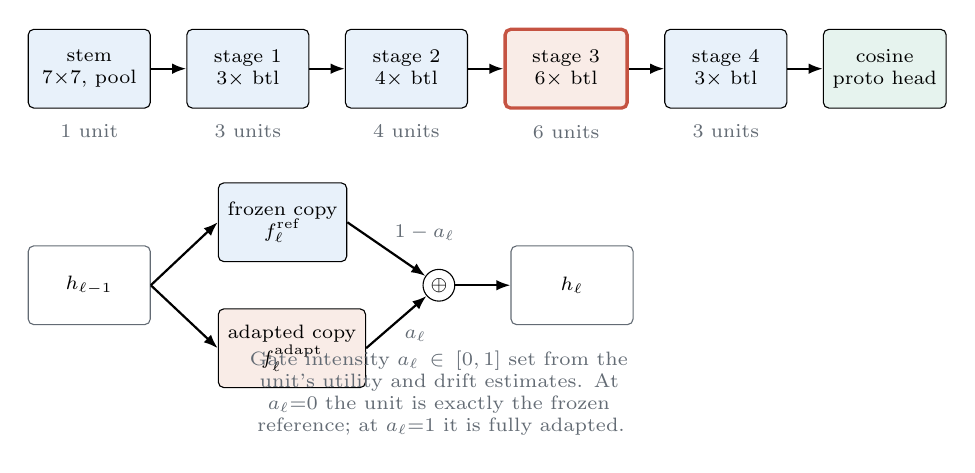
\begin{tikzpicture}[
  stage/.style={draw,rounded corners=2pt,align=center,minimum width=1.55cm,minimum height=1.0cm,font=\scriptsize},
  tiny/.style={font=\scriptsize,midgray},
  arr/.style={-{Latex[length=1.8mm]},thick}
]
\node[stage,fill=lightblue] (stem) {stem\\\scriptsize $7{\times}7$, pool};
\node[stage,fill=lightblue,right=0.45cm of stem] (s1) {stage 1\\\scriptsize $3\times$ btl};
\node[stage,fill=lightblue,right=0.45cm of s1] (s2) {stage 2\\\scriptsize $4\times$ btl};
\node[stage,fill=lightorange,right=0.45cm of s2,draw=mlpcol,very thick] (s3) {stage 3\\\scriptsize $6\times$ btl};
\node[stage,fill=lightblue,right=0.45cm of s3] (s4) {stage 4\\\scriptsize $3\times$ btl};
\node[stage,fill=lightgreen,right=0.45cm of s4] (head) {cosine\\proto head};
\foreach \a/\b in {stem/s1,s1/s2,s2/s3,s3/s4,s4/head}{\draw[arr] (\a)--(\b);}
\node[tiny,below=0.08cm of stem] {1 unit};
\node[tiny,below=0.08cm of s1] {3 units};
\node[tiny,below=0.08cm of s2] {4 units};
\node[tiny,below=0.08cm of s3] {6 units};
\node[tiny,below=0.08cm of s4] {3 units};

\begin{scope}[shift={(0,-2.75cm)}]
  \node[stage,fill=white,draw=midgray] (hin) {$h_{\ell-1}$};
  \node[stage,fill=lightblue,right=0.85cm of hin,yshift=0.80cm] (froz) {frozen copy\\\scriptsize $f^{\mathrm{ref}}_\ell$};
  \node[stage,fill=lightorange,right=0.85cm of hin,yshift=-0.80cm] (adap) {adapted copy\\\scriptsize $f^{\mathrm{adapt}}_\ell$};
  \node[draw,circle,inner sep=1.2pt,right=0.85cm of hin,xshift=2.6cm,font=\scriptsize] (mix) {$\oplus$};
  \node[stage,fill=white,draw=midgray,right=0.7cm of mix] (hout) {$h_\ell$};
  \draw[arr] (hin.east)--(froz.west); \draw[arr] (hin.east)--(adap.west);
  \draw[arr] (froz.east)-- node[tiny,above right=-1pt]{$1-a_\ell$} (mix);
  \draw[arr] (adap.east)-- node[tiny,below right=-1pt]{$a_\ell$} (mix);
  \draw[arr] (mix)--(hout);
  \node[tiny,below=0.5cm of mix,align=center,text width=5.6cm]
    {Gate intensity $a_\ell\in[0,1]$ set from the unit's utility and drift
     estimates. At $a_\ell{=}0$ the unit is exactly the frozen reference; at
     $a_\ell{=}1$ it is fully adapted.};
\end{scope}
\end{tikzpicture}
\caption{The ResNet-50 pilot. \textbf{Top:} the backbone is divided into
seventeen controllable units, the stem plus each of the sixteen bottleneck
blocks, which is the granularity the ARC controller operated on. One stage is
outlined to indicate where a selected unit sits; the controller assigned an
intensity to every unit rather than choosing one. Stage widths
and spatial resolutions differ between stages, which is precisely why this
architecture cannot isolate depth as cleanly as a ViT whose blocks are
structurally identical. \textbf{Bottom:} the per-unit gate. Each unit runs a
frozen reference copy and an episode-adapted copy, and their outputs are
interpolated by the learned intensity $a_\ell$. The measured gate stayed high
enough that $84$--$98\%$ of parameters were still modified, so the intended
sparse adaptation was never realised.}
\label{fig:resnetarch}
\end{figure}

The ResNet pilot produced three relevant observations. First, the tuned adaptive gate did not improve over the fixed adaptation baselines. Second, its sigmoid gate often remained high, so it still modified most of the backbone and did not realize its intended sparse-adaptation behaviour. Third, the tested signals did not reliably rank units according to their realised adaptation benefit. These findings do not show that all representation-aware controllers are ineffective. They show that this particular signal-and-gate implementation did not supply evidence to justify the more expensive extensions.

The subsequent ViT experiments remove the controller and directly intervene on a selected block. That design serves two purposes: it tests whether placement itself has a large effect, and it avoids conflating the effect of depth with the controller's signal quality. The ResNet findings below are reported as exploratory pilot results and as the motivation for the pivot; the primary claims in this paper come from the controlled ViT depth sweeps.

\subsection{Tasks and datasets}

We study EuroSAT and ISIC 2018 as target domains; \cref{tab:datasets} summarises the two partitions. EuroSAT contains 27,000 RGB satellite-image tiles across ten land-use and land-cover categories \cite{helber2019}. ISIC 2018 Task 3 uses the HAM10000 dermoscopic image collection, containing 10,015 images across seven diagnostic categories \cite{tschandl2018,codella2019}. The two datasets differ in visual content and acquisition process. We use them to demonstrate that the depth profile is not identical across target datasets; we do not treat two datasets as a sufficient sample for estimating a general relationship between a numerical measure of domain shift and optimal depth.

The fixed split seed is 0. EuroSAT is split into train/validation/test fractions of 0.2/0.1/0.7, containing 5,400, 2,700, and 18,900 images respectively. ISIC uses fractions of 0.1/0.4/0.5, containing 1,000, 4,013, and 5,002 images respectively. The fractions differ because the ISIC class distribution is substantially imbalanced: a split with a smaller validation allocation leaves too few samples in the rarest categories to form the intended episodic tasks. We chose the fractions after checking per-class episode feasibility rather than forcing identical percentages across datasets.

ISIC is partitioned by lesion identifier using the HAM10000 metadata, not by image filename alone. The 10,015 images correspond to 7,470 lesion IDs. The group-disjoint partition assigns 747, 2,988, and 3,735 lesion groups to train, validation, and test respectively. This prevents views of the same lesion from being placed on opposite sides of a split, a leakage risk in datasets where some physical lesions are photographed more than once. For EuroSAT, each tile is treated as an independent sample; group-disjoint splitting consequently reduces to a random image split.

\begin{table}[t]
\centering
\small
\caption{Target datasets and partitions used in the ViT experiments. All headline values reported in this manuscript come from the validation split.}
\label{tab:datasets}
\begin{tabularx}{\textwidth}{lYrrrl}
\toprule
Dataset & Domain / labels & Train images & Validation images & Test images & Split unit\\
\midrule
EuroSAT & Satellite RGB; 10 classes & 5,400 & 2,700 & 18,900 & Image tile\\
ISIC 2018 & Dermoscopy; 7 classes & 1,000 & 4,013 & 5,002 & Lesion ID\\
\bottomrule
\end{tabularx}
\end{table}

\subsection{Episodic protocol}

The main evaluation uses 5-way 5-shot episodes with 15 query examples per class. Each episode therefore contains 25 labelled support examples and 75 query examples. The support set is used for episode-specific adaptation; predictions are measured on query examples not used in that episode's support loss. The main depth experiments use 100 episodes for each of three episode-sampling seeds, 0, 1, and 2, with the data split fixed at seed 0. Each compared method uses the same episode indices within a seed, enabling paired comparisons.

The evaluation pipeline uses a cosine-distance Prototypical Network head \cite{snell2017}. Given an embedding function $f_\theta$, the prototype for class $c$ is
\begin{equation}
 \mathbf{p}_c=\frac{1}{|S_c|}\sum_{(x_i,y_i)\in S_c,\,y_i=c} f_\theta(x_i),
\end{equation}
and query predictions are based on cosine similarity between the query embedding and each support-derived prototype. The backbone's selected parameter group is updated for 20 inner-loop Adam steps under the episode support objective, after which query classification uses the cosine prototype head. Frozen-backbone ProtoNet is the no-gradient reference condition. Hyperparameters for each adaptation baseline were tuned on validation; the held-out test split was not read during tuning and no test-split accuracy is claimed in this manuscript.

\subsection{Backbone and parameter groups}

\Cref{fig:vitintervention} shows the intervention schematically and \cref{tab:vitgroups} lists the resulting groups. The primary backbone is a ViT-B/16 model with the public supervised ImageNet-21k AugReg initialization distributed as \method{vit\_base\_patch16\_224.augreg\_in21k} \cite{vit2021,steiner2022}. It has twelve transformer blocks and 85,798,656 parameters in the parameter partition used by the experiments. The architecture makes depth a relatively clean factor: each block contains an attention sublayer and an MLP sublayer of the same dimensions. The selected block is varied while the family and nominal parameter count are fixed.

\begin{figure}[t]
\centering
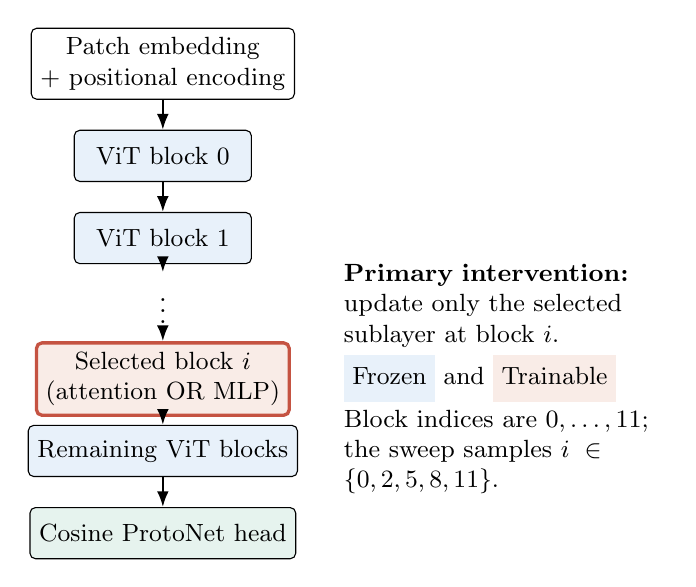
\begin{tikzpicture}[
  block/.style={draw,rounded corners=2pt,minimum width=2.25cm,minimum height=0.65cm,align=center,font=\small},
  freeze/.style={block,fill=lightblue},
  train/.style={block,fill=lightorange,draw=mlpcol,very thick},
  arr/.style={-{Latex[length=2mm]},thick},
  node distance=0.38cm
]
\node[block,fill=white] (patch) {Patch embedding\\+ positional encoding};
\node[freeze,below=of patch] (b0) {ViT block 0};
\node[freeze,below=of b0] (b1) {ViT block 1};
\node[below=0.1cm of b1] (dots) {$\vdots$};
\node[train,below=0.1cm of dots] (bi) {Selected block $i$\\(attention OR MLP)};
\node[freeze,below=0.1cm of bi] (bn) {Remaining ViT blocks};
\node[block,fill=lightgreen,below=of bn] (head) {Cosine ProtoNet head};
\draw[arr] (patch)--(b0); \draw[arr] (b0)--(b1); \draw[arr] (b1)--(dots); \draw[arr] (dots)--(bi); \draw[arr] (bi)--(bn); \draw[arr] (bn)--(head);
\node[align=left,font=\small,right=0.55cm of bi,text width=4.0cm] (key) {\textbf{Primary intervention:} update only the selected sublayer at block $i$.\\[0.2em]
\colorbox{lightblue}{\strut Frozen} and \colorbox{lightorange}{\strut Trainable}\\[0.2em]
Block indices are $0,\ldots,11$; the sweep samples $i\in\{0,2,5,8,11\}$.};
\end{tikzpicture}
\caption{A schematic of the ViT intervention used in the depth experiments. Unlike the standard encoder--decoder Transformer diagram used in some sequence-to-sequence papers, the evaluated vision model is an encoder-only ViT. The highlight denotes the sublayer whose parameters are updated for a single-block run; all other backbone weights are frozen.}
\label{fig:vitintervention}
\end{figure}

The primary parameter groups are:
\begin{itemize}
  \item \method{attn\_only\_ft}: attention projection parameters from all twelve blocks (28,348,416 parameters, 33.041\% of the backbone).
  \item \method{mlp\_only\_ft}: MLP parameters from all twelve blocks (56,669,184 parameters, 66.049\%).
  \item \method{ln\_only\_ft}: all LayerNorm affine parameters (38,400 parameters, 0.045\%). The scale and shift subsets each contain 19,200 parameters (about 0.022\%).
  \item \method{patch\_embed\_ft}: patch-embedding parameters (742,656 parameters, 0.866\%).
  \item \method{full\_ft}: all 85,798,656 parameters.
\end{itemize}

An individual attention block contains approximately 2.75\% of the model parameters; an individual MLP block contains approximately 5.50\%. The selector tests assert that all single-block attention selections have the same parameter count, and analogously for MLP. This equality is essential to interpreting a depth sweep as a positional comparison rather than a hidden capacity comparison. The selected positions are blocks 0, 2, 5, 8, and 11; the study does not measure every one of the twelve positions.

\subsection{Experimental pipeline}

\Cref{fig:pipeline} summarizes the end-to-end evaluation path used for every reported configuration: a fixed split of the target dataset, the pretrained checkpoint, a choice of adaptation family and depth, episode sampling, the inner-loop update restricted to the selected weights, and cosine-prototype scoring of held-out query images. Only the selected parameters receive gradients; the test partition is untouched throughout.

\begin{figure}[t]
\centering
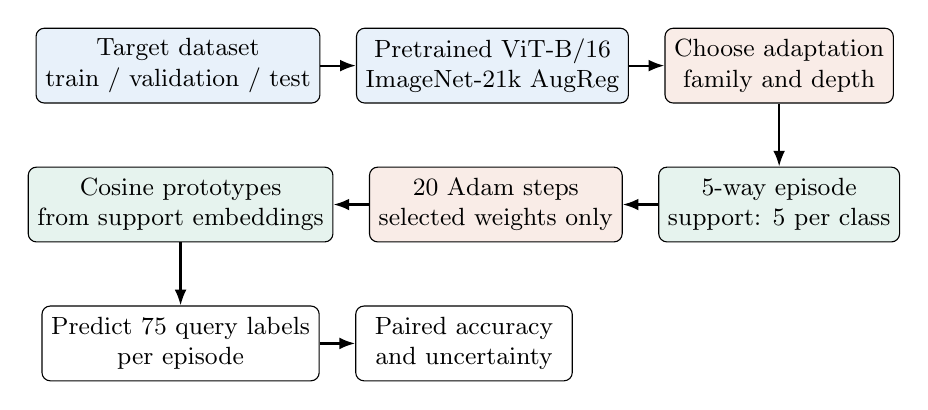
\begin{tikzpicture}[
  box/.style={draw,rounded corners=3pt,align=center,minimum width=2.75cm,minimum height=0.95cm,font=\small},
  arr/.style={-{Latex[length=2mm]},thick},
  node distance=0.8cm and 0.45cm
]
\node[box,fill=lightblue] (data) {Target dataset\\train / validation / test};
\node[box,fill=lightblue,right=of data] (pre) {Pretrained ViT-B/16\\ImageNet-21k AugReg};
\node[box,fill=lightorange,right=of pre] (select) {Choose adaptation\\family and depth};
\node[box,fill=lightgreen,below=of select] (episode) {5-way episode\\support: 5 per class};
\node[box,fill=lightorange,left=of episode] (update) {20 Adam steps\\selected weights only};
\node[box,fill=lightgreen,left=of update] (proto) {Cosine prototypes\\from support embeddings};
\node[box,fill=white,below=of proto] (query) {Predict 75 query labels\\per episode};
\node[box,fill=white,right=of query] (stats) {Paired accuracy\\and uncertainty};
\draw[arr] (data)--(pre); \draw[arr] (pre)--(select); \draw[arr] (select)--(episode); \draw[arr] (episode)--(update); \draw[arr] (update)--(proto); \draw[arr] (proto)--(query); \draw[arr] (query)--(stats);
\end{tikzpicture}
\caption{End-to-end evaluation pipeline. The test partition remains untouched during hyperparameter tuning and all values in this paper are validation results.}
\label{fig:pipeline}
\end{figure}

\subsection{Learning-rate selection and edge handling}

Learning rates are not shared across parameter groups. Updating a small parameter family generally requires a different learning-rate scale from updating the whole network, and the initial ResNet experiments showed that a shared learning rate can make a parameter-family comparison uninterpretable. We use a logarithmic grid and choose each group's setting on validation. If the best candidate lies at the upper or lower edge of the grid, that result is treated as a boundary rather than an optimum and the grid is extended where appropriate. For the depth and MLP comparisons, the tuned settings are then held fixed for the additional episode-sampling seeds, so the replicated curves vary the episode sample rather than retuning every cell for each draw.

This procedure does not eliminate all selection bias: choosing the learning rate based on validation accuracy makes validation a model-selection resource. It does, however, keep the test split isolated and makes explicit that reported results describe performance under validation-tuned adaptation settings. The learning-rate sweeps use 50 episodes per configuration to identify candidate settings; the main reported depth curves are re-evaluated on 100 episodes per draw.

\subsection{Primary depth interventions}

\begin{algorithm}[t]
\caption{Episodic depth intervention. One evaluated configuration is the triple
(parameter family $\mathcal{F}$, block index $i$, learning rate $\eta$). The
backbone is restored from the pretrained snapshot before every episode, so no
information crosses episode boundaries.}
\label{alg:depth}
\begin{algorithmic}[1]
\Require pretrained backbone $\theta_0$; family $\mathcal{F}\in\{\textsc{attn},\textsc{mlp}\}$;
block $i$; rate $\eta$; steps $T{=}20$; episodes $N{=}100$; draw seed $s$
\Ensure mean query accuracy over the draw
\State $\mathcal{S}\gets$ parameter indices of family $\mathcal{F}$ in block $i$
\Comment{all other backbone weights stay frozen}
\For{$n = 1$ \textbf{to} $N$}
  \State $\theta \gets \theta_0$ \Comment{restore; episodes never share state}
  \State $(S, Q) \gets \textsc{SampleEpisode}(\text{val split}, \text{seed}{=}h(s,n))$
  \Comment{5-way, 5 support, 15 query per class}
  \For{$t = 1$ \textbf{to} $T$}
    \State $\mathbf{p}_c \gets \frac{1}{|S_c|}\sum_{x\in S_c} f_\theta(x)$ for each class $c$
    \State $\mathcal{L} \gets \textsc{SupportLoss}\big(\{f_\theta(x)\}_{x\in S}, \{\mathbf{p}_c\}\big)$
    \State $\theta_{\mathcal{S}} \gets \textsc{Adam}(\theta_{\mathcal{S}}, \nabla_{\theta_{\mathcal{S}}}\mathcal{L}, \eta)$
    \Comment{gradients restricted to $\mathcal{S}$}
  \EndFor
  \State $\mathbf{p}_c \gets \frac{1}{|S_c|}\sum_{x\in S_c} f_\theta(x)$
  \Comment{prototypes recomputed after adaptation}
  \State $a_n \gets \textsc{Accuracy}\big(\arg\max_c \cos(f_\theta(q), \mathbf{p}_c),\; y_Q\big)$
\EndFor
\State \Return $\frac{1}{N}\sum_n a_n$
\end{algorithmic}
\end{algorithm}


\Cref{alg:depth} states the procedure evaluated for every configuration. For a depth index $i$, let $\method{attn\_block}_i$ denote a model in which only the attention projections in ViT block $i$ are updated, and let $\method{mlp\_block}_i$ denote the corresponding MLP-only intervention. Each single-block model is compared to frozen ProtoNet and full fine-tuning. Because the parameter family and count are constant across $i$ within each sweep, the difference
\begin{equation}
 \Delta_{i,j}=\operatorname{Acc}(i)-\operatorname{Acc}(j)
\end{equation}
measures the outcome difference for moving the adaptation location between tested blocks, under the selected hyperparameters and episode distribution.

Because $h(s,n)$ depends only on the draw seed and the episode index,
every configuration compared within a draw sees \emph{identical} episodes. All
reported differences are therefore paired at the episode level, which removes
episode-difficulty variance from the comparison. The learning rate $\eta$ is the
only quantity tuned per configuration, and it is tuned on validation; the test
split is never read.

The depth study addresses four descriptive questions:
\begin{enumerate}
  \item Is the accuracy curve approximately flat or does it vary materially with depth?
  \item Does the profile change between attention and MLP adaptation?
  \item Does the profile transfer across the two target datasets, or does the preferred region change?
  \item Does a single-block intervention beat whole-network fine-tuning, and if so, on which dataset and at which tested locations?
\end{enumerate}

\subsection{Mechanism probes}

Three follow-up experiments investigate a capacity-versus-data explanation for why single-block adaptation can beat full fine-tuning on EuroSAT at five shots.

\paragraph{Inner-loop length.} The attention-only and full fine-tuning baselines are evaluated at 5, 10, and 20 inner steps. Each step-count condition receives its own learning-rate tuning so that a result is not merely caused by one method being more sensitive to an inappropriate step size. This probe has one episode draw and is interpreted as directional evidence rather than a replicated multi-seed estimate.

\paragraph{Support-set size.} EuroSAT is evaluated at $k\in\{1,5,20\}$ shots per class. The main five-shot benchmark has three draws; the matched support-size follow-up at each of $k=1,5,20$ uses one draw with common episodes across attention-only, full fine-tuning, and a frozen reference. We compare each adapted method with frozen ProtoNet as well as comparing the two adapted methods. At twenty shots, both adapted methods reach about 94\% accuracy, but the frozen reference is 86.35\%, so this is not simply a ceiling case in which adaptation has no effect. The revised gain-over-frozen statistic was specified after seeing the lower-shot outcomes; the twenty-shot row is its prospective check and must be interpreted as limited evidence, not a fully replicated mechanism test.

\paragraph{Weight decay.} Weight decay is tested at $0,10^{-4},10^{-3},10^{-2},10^{-1}$ for full fine-tuning and attention-only adaptation. Differences are paired against each method's own zero-decay condition on the same episodes. The implementation uses Adam with coupled L2 penalty; it is not decoupled AdamW. Moreover, the two baselines use separately tuned learning rates. Accordingly, the within-baseline dose response is easier to interpret than differences in nominal regularization strength across the two baselines. The tested intervention pulls weights toward zero, not toward the pretrained initialization; an $\ell_2$-SP-style penalty to the initial weights was not run.

\subsection{Statistics and reproducibility}

For the replicated depth curves, we report the mean and standard deviation of accuracy across the three episode-sampling seeds. For pairwise comparisons, the same episodes are used for the two methods within each seed. The three per-seed paired differences are summarized as
\begin{equation}
 \bar d \pm t_{0.975,2}\frac{s_d}{\sqrt{3}}, \qquad t_{0.975,2}=4.303.
 \label{eq:pairedci}
\end{equation}
These intervals summarize variability over three episode-draw seeds; with only three seeds they should not be mistaken for a precise population-level uncertainty estimate. For single-draw paired comparisons, the episode-level paired differences are summarized with a $t$ interval over the 100 episodes. We distinguish these two cases in the tables and text.

Repeated identical fine-tuning runs can differ by roughly 0.6 percentage points because nondeterminism in GPU backward and optimizer execution is amplified during Adam updates. A frozen backbone is exactly reproducible under the measured configuration. We therefore avoid strong interpretations of small single-run gaps near or below this level. This floor is a practical diagnostic, not a universal statistical threshold. The three-draw paired estimates are preferred for the main depth claims.

\section{Exploratory ResNet-50 investigation}
\label{sec:resnet}

The ResNet-50 arm both motivated ARC and exposed why a more controlled depth study was needed. Because ResNet stages and units differ in spatial resolution, width, and parameter count, a naive layer comparison on this architecture would not isolate depth as cleanly as a ViT block comparison. The ResNet results are therefore reported as an exploratory pilot and not combined numerically with the ViT results.

\subsection{Tuned baselines on EuroSAT}

\Cref{tab:resnetbaseline} reports the initial baseline evaluation, which compared frozen ProtoNet, last-layer tuning, BatchNorm-only tuning, stage-4 tuning, progressive unfreezing, and full fine-tuning. Each trainable baseline was tuned on validation. The 1-shot and 5-shot cells pooled three episode-sampling seeds; the 10-shot and 20-shot cells pooled two seeds and are shown only as context.

\begin{table}[t]
\centering
\small
\caption{ResNet-50 EuroSAT validation baselines from the exploratory ARC arm. Values are mean accuracy with 95\% episode-level intervals as recorded by the experiment runner. The 10-shot and 20-shot entries use two draws; the other entries use three.}
\label{tab:resnetbaseline}
\begin{tabular}{lrrrr}
\toprule
Method & 1-shot & 5-shot & 10-shot & 20-shot\\
\midrule
Frozen ProtoNet & 67.67 $\pm$ 0.47 & 84.59 $\pm$ 0.29 & 87.28 $\pm$ 0.32 & 88.99 $\pm$ 0.27\\
Last-layer FT & 67.70 $\pm$ 0.47 & 84.80 $\pm$ 0.29 & 89.11 $\pm$ 0.30 & 91.99 $\pm$ 0.24\\
BatchNorm-only FT & 68.46 $\pm$ 0.49 & 86.83 $\pm$ 0.29 & 90.79 $\pm$ 0.27 & 93.61 $\pm$ 0.20\\
Stage-4 FT & 69.06 $\pm$ 0.48 & 87.73 $\pm$ 0.27 & 91.11 $\pm$ 0.26 & 93.51 $\pm$ 0.21\\
Progressive unfreezing & 68.51 $\pm$ 0.48 & 87.66 $\pm$ 0.27 & 91.06 $\pm$ 0.26 & 93.64 $\pm$ 0.20\\
Full FT & 68.37 $\pm$ 0.48 & 87.21 $\pm$ 0.28 & 91.35 $\pm$ 0.26 & 94.02 $\pm$ 0.20\\
\bottomrule
\end{tabular}
\end{table}

At five shots, the frozen reference reaches 84.59\%, stage-4 tuning reaches 87.73\%, and full fine-tuning reaches 87.21\%. This was an early indication that updating more parameters was not automatically better on EuroSAT. The result alone does not isolate depth from parameter count or update dynamics, which is why the subsequent ViT sweep is more controlled.

On ISIC, ResNet-50 full fine-tuning achieved 49.55\% at five shots, compared with 49.44\% for BatchNorm-only fine-tuning. BatchNorm-only training updates approximately 0.22\% of parameters. This near-tie is important as an exploratory observation, but it is not a direct estimate of the expected ViT LayerNorm effect: the architectures differ, BatchNorm and LayerNorm have different operational properties, and all values are validation results.

\subsection{The adaptive gate did not provide a measurable advantage}

The first implemented ARC gate used utility $U_\ell$ and drift $D_\ell$ to set an adaptation intensity. Drift was computed from the difference between activations of the frozen reference and adapted network; the intended gate should have assigned lower adaptation intensity to units whose adaptation was less useful or excessively disruptive. The gate's coefficients were treated as validation-tuned hyperparameters rather than learned parameters, because a gate that only masks gradients does not receive a useful coefficient gradient through the masked-gradient path.

Across EuroSAT and ISIC, the marginal effects of the tested utility and drift signals were neutral or negative (\cref{tab:gate}). On EuroSAT, utility's marginal effect was approximately $-0.05$ points at one shot and $+0.04$ at five shots; drift was $-0.10$ and $-1.20$ points, respectively. On ISIC the corresponding effects were $-0.18$ and $-1.43$ for utility, and $-0.30$ and $-3.33$ for drift. The gate's average intensity remained high enough that approximately 84--98\% of parameters were still modified, so the implementation did not create a genuinely sparse update. Comparing the best configuration from a larger signal-enabled sweep with the best from a smaller signal-disabled sweep would favour the larger search space; the marginal effects above are more appropriate summaries.

\begin{table}[t]
\centering
\small
\caption{Marginal effects of the tested ARC gate signals, in percentage points. These are validation results from the ResNet-50 pilot, not the main ViT experiment.}
\label{tab:gate}
\begin{tabular}{lrrrr}
\toprule
Signal & EuroSAT 1-shot & EuroSAT 5-shot & ISIC 1-shot & ISIC 5-shot\\
\midrule
Utility $U$ & $-0.05$ & $+0.04$ & $-0.18$ & $-1.43$\\
Drift $D$ & $-0.10$ & $-1.20$ & $-0.30$ & $-3.33$\\
\bottomrule
\end{tabular}
\end{table}

The null gate result changed the project plan. The expensive topological, stability, novelty, and stochastic-control extensions were not executed in the final experimental programme. It would be inaccurate to describe the full five-signal or FBSDE controller as experimentally validated. The defensible statement is that the tested two-signal gate did not improve reliably, its parameter-efficiency objective was not realized, and further controller complexity was not justified before understanding what the signals should control.

\subsection{Representation displacement and unit-level diagnostics}

Follow-up ResNet diagnostics examined whether full fine-tuning's activation displacement was structurally complex. A per-channel affine transformation accounted for approximately 90\% of the measured displacement in selected activation probes, suggesting that some of the change could be represented with scale-and-shift corrections. This is a descriptive activation-space decomposition; it does not imply that a per-channel affine reproduces the whole fine-tuned function or that a fixed affine extracted on one support/query batch generalizes to unseen episodes.

The unit-benefit probe compared each unit's stand-alone adaptation gain and its marginal contribution when other units were already adapted. The sum of stand-alone unit gains substantially exceeded the gain from adapting all units together, while removing a unit from a jointly adapted model often had little effect. This pattern is consistent with redundancy or interference among unit updates. However, the probe was run over a relatively small number of episodes and is not strong enough to rank small unit benefits precisely. The utility and drift signals did not reliably predict the measured benefit of adapting a unit. Drift also tracked depth strongly in the observed configuration, raising the possibility that it behaved more like a fixed depth indicator than a genuinely episode-specific signal.

A precomputed correction experiment estimated an affine activation correction from full fine-tuning displacements and applied it without gradient steps. Its results were variable across extraction runs, particularly in the shallower units where the estimated displacement was smaller. On ISIC, the whole-network shift correction provided only a small gain over frozen ProtoNet and showed a roughly two-point spread between two extracted corrections. Further comparisons found that a per-channel scale-and-shift variant outperformed some low-rank displacement variants in that particular probe, while the reverse was not reliably established across datasets. These measurements are retained as exploratory diagnostics, not as a central performance claim. Their practical lesson is methodological: a precomputed activation correction must account for uncertainty in how its displacement basis is estimated, rather than reporting only query-episode uncertainty.

\section{Main ViT results}
\label{sec:results}

\subsection{The main comparison across parameter families}

Before isolating depth, we evaluate several broad parameter groups at their individually tuned validation learning rates. The three-draw reference results for the parameter groups that received full replication are summarized in \cref{tab:vitgroups}. Group-level values for patch embedding and some scale/shift variants come from a single draw and are identified as such; they should not be read as equally replicated with the main attention/full/frozen comparisons.

\begin{table}[t]
\centering
\small
\caption{ViT-B/16 parameter-family results on validation. Replicated values show mean accuracy and standard deviation across three episode draws; cells marked $^\dagger$ are single-draw values. Percentages denote the nominal fraction of backbone parameters selected for updating, not necessarily the fraction that moved by a numerically nonzero amount.}
\label{tab:vitgroups}
\begin{tabular}{llrr}
\toprule
Dataset & Parameter group & Trainable parameters & Accuracy (\%)\\
\midrule
EuroSAT & Frozen ProtoNet & 0 & 79.22 $\pm$ 0.26\\
EuroSAT & Patch embedding FT$^\dagger$ & 742,656 (0.866\%) & 79.44\\
EuroSAT & LayerNorm-only FT & 38,400 (0.045\%) & 84.18 $\pm$ 0.51\\
EuroSAT & MLP-only FT & 56,669,184 (66.049\%) & 84.38\\
EuroSAT & Attention-only FT & 28,348,416 (33.041\%) & 85.56 $\pm$ 0.35\\
EuroSAT & Full FT & 85,798,656 (100\%) & 83.07 $\pm$ 0.20\\
\midrule
ISIC & Frozen ProtoNet & 0 & 38.26 $\pm$ 0.98\\
ISIC & LayerNorm-only FT & 38,400 (0.045\%) & 48.91 $\pm$ 0.61\\
ISIC & Attention-only FT & 28,348,416 (33.041\%) & 49.29 $\pm$ 0.82\\
ISIC & Full FT & 85,798,656 (100\%) & 51.50 $\pm$ 0.87\\
\bottomrule
\end{tabular}
\end{table}

On EuroSAT, attention-only tuning is the strongest replicated whole-family baseline, at 85.56\%, while full fine-tuning averages 83.07\%. The paired difference across episode seeds is $+2.50\pm0.64$ points in favour of attention-only adaptation. The frozen reference is 79.22\%, so the attention-only gain is approximately 6.34 points, against approximately 3.85 points for full fine-tuning. LayerNorm-only adaptation is much smaller and reaches 84.18\%, which is close to the strongest family-level result for a parameter fraction of 0.045\%.

On ISIC, the ordering changes. Full fine-tuning averages 51.50\%, ahead of attention-only tuning at 49.29\% by a paired $2.20\pm0.30$ points. The LayerNorm-only result is 48.91\%. This is consistent with the premise that domain shift affects how much model capacity is useful, but it is not itself proof of a causal relationship with a measured shift magnitude. In particular, two datasets cannot establish a monotonic law relating shift magnitude to full fine-tuning's benefit.

\Cref{fig:paramsacc} plots these families against the fraction of the backbone they update, together with the two best single-block interventions. Accuracy is visibly non-monotonic in parameter count: the ordering of configurations is not recoverable from size alone, which is what motivates treating position as its own variable. The family table motivates the depth comparison, but it is not a controlled ranking of every PEFT method in the literature. Each parameter group has its own tuned learning rate, and some groups have fewer draws than the main curves. Published results for SSF, LN-Tune, DIPA, or other methods were not rerun under this exact backbone, pretraining, split, and episodic protocol; they are discussed conceptually in \cref{sec:related}, not compared numerically against \cref{tab:vitgroups}.

\begin{figure}[t]
\centering
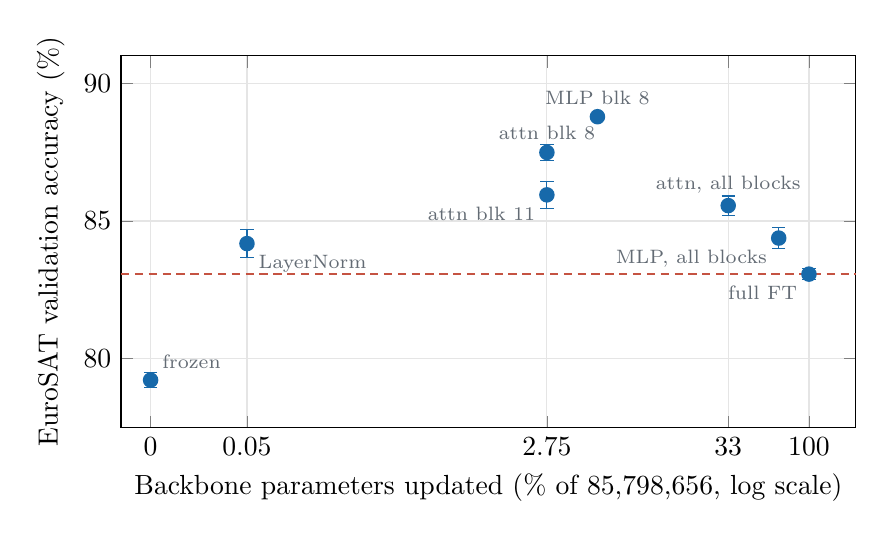
\begin{tikzpicture}
\begin{axis}[
 width=0.90\textwidth,height=6.3cm,
 xmode=log,log basis x=10,
 xlabel={Backbone parameters updated (\% of 85{,}798{,}656, log scale)},
 ylabel={EuroSAT validation accuracy (\%)},
 xmin=0.008,xmax=190,ymin=77.5,ymax=91.0,
 grid=major,grid style={gray!20},
 xtick={0.012,0.045,2.75,33.04,100},
 xticklabels={$0$,$0.05$,$2.75$,$33$,$100$},
 every axis plot/.append style={thick}
]
\addplot[only marks,attncol,mark=*,mark size=2.4pt,error bars/.cd,y dir=both,y explicit] coordinates {
  (0.012,79.22) +- (0,0.26)
  (0.045,84.18) +- (0,0.51)
  (2.75,87.49) +- (0,0.29)
  (2.75,85.95) +- (0,0.50)
  (5.5,88.79) +- (0,0.11)
  (33.04,85.56) +- (0,0.35)
  (66.05,84.38) +- (0,0.39)
  (100.0,83.07) +- (0,0.20)
};
\addplot[mlpcol,densely dashed,thick,domain=0.008:190,samples=2]{83.07};
\node[font=\scriptsize,above right=1pt,midgray] at (axis cs:0.012,79.22) {frozen};
\node[font=\scriptsize,below right=1pt,midgray] at (axis cs:0.045,84.18) {LayerNorm};
\node[font=\scriptsize,above=1pt,midgray] at (axis cs:2.75,87.49) {attn blk 8};
\node[font=\scriptsize,below left=1pt,midgray] at (axis cs:2.75,85.95) {attn blk 11};
\node[font=\scriptsize,above=1pt,midgray] at (axis cs:5.5,88.79) {MLP blk 8};
\node[font=\scriptsize,above=1pt,midgray] at (axis cs:33.04,85.56) {attn, all blocks};
\node[font=\scriptsize,below left=1pt,midgray] at (axis cs:66.05,84.38) {MLP, all blocks};
\node[font=\scriptsize,below left=1pt,midgray] at (axis cs:100.0,83.07) {full FT};
\end{axis}
\end{tikzpicture}
\caption{Accuracy against the fraction of backbone parameters updated, EuroSAT
validation, three episode draws, error bars one standard deviation. The dashed
line is full fine-tuning. Accuracy is not monotonic in parameter count: a single
attention block at $2.75\%$ and a single MLP block at $5.50\%$ both sit above
the $100\%$ point, while a differently placed block of identical size does not.
Parameter count alone therefore does not order these configurations.}
\label{fig:paramsacc}
\end{figure}

\subsection{Attention depth on EuroSAT}
\label{sec:attndepth}

The five tested single-block attention interventions show a pronounced depth profile, plotted in \cref{fig:depthcurves} and tabulated with the MLP and ISIC sweeps in \cref{tab:depthmeans}. Across three episode draws, the average accuracy is 78.76\% at block 0, 78.64\% at block 2, 81.78\% at block 5, 87.49\% at block 8, and 85.95\% at block 11. The standard deviation across the three draws ranges from 0.29 to 0.50 points. Block 8 is the peak of the measured curve in all three draws, though the experiment does not locate the optimum among untested blocks 6, 7, 9, or 10.

\begin{figure}[t]
\centering
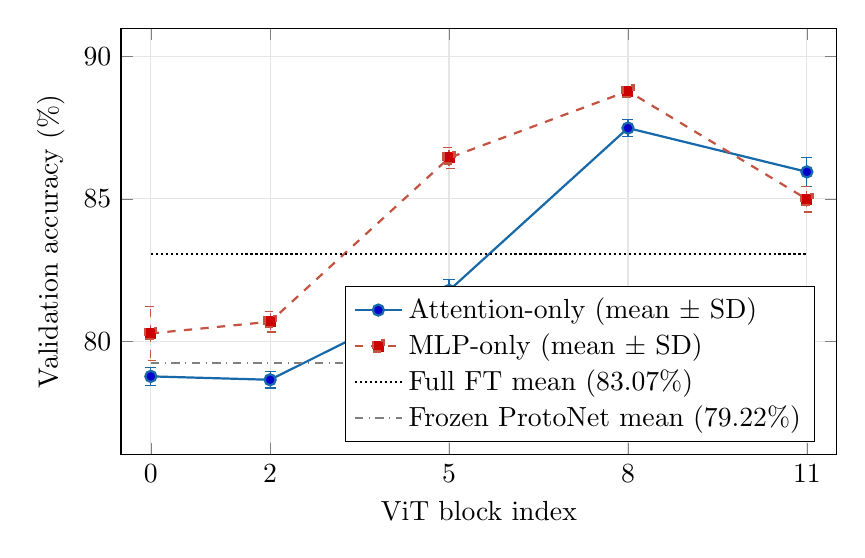
\begin{tikzpicture}
\begin{axis}[
 width=0.88\textwidth,height=7cm,
 xlabel={ViT block index},ylabel={Validation accuracy (\%)},
 xtick={0,2,5,8,11},xmin=-0.5,xmax=11.5,ymin=76,ymax=91,
 grid=major,grid style={gray!20},legend pos=south east,legend cell align=left,
 error bars/y dir=both,error bars/y explicit
]
\addplot+[attncol,mark=*,thick,error bars/.cd,y dir=both,y explicit] coordinates {
 (0,78.76) +- (0,0.32)
 (2,78.64) +- (0,0.29)
 (5,81.78) +- (0,0.39)
 (8,87.49) +- (0,0.29)
 (11,85.95) +- (0,0.50)
};
\addlegendentry{Attention-only (mean $\pm$ SD)}
\addplot+[mlpcol,mark=square*,thick,dashed,error bars/.cd,y dir=both,y explicit] coordinates {
 (0,80.27) +- (0,0.96)
 (2,80.68) +- (0,0.36)
 (5,86.44) +- (0,0.36)
 (8,88.79) +- (0,0.11)
 (11,84.99) +- (0,0.45)
};
\addlegendentry{MLP-only (mean $\pm$ SD)}
\addplot[black,densely dotted,thick,domain=0:11,samples=2]{83.07};
\addlegendentry{Full FT mean (83.07\%)}
\addplot[gray,dashdotted,thick,domain=0:11,samples=2]{79.22};
\addlegendentry{Frozen ProtoNet mean (79.22\%)}
\end{axis}
\end{tikzpicture}
\caption{EuroSAT validation depth profiles. Error bars are one standard deviation across three episode-sampling seeds, not 95\% confidence intervals. Block 8 is the best of the five tested positions for both parameter families.}
\label{fig:depthcurves}
\end{figure}

The depth span for attention-only adaptation is 8.89, 9.31, and 8.41 percentage points in the three draws, respectively (mean span 8.85). The shallow pair (blocks 0 and 2) is indistinguishable at the scale of these draws: the paired cross-seed estimate for block 2 minus block 0 is $-0.12\pm0.48$. By contrast, block 8 exceeds block 5 by $5.71\pm1.38$ and block 11 by $1.54\pm0.80$ in the paired three-draw comparison. It also exceeds a suffix adaptation using the final six attention blocks, which contains block 8, by $1.26\pm0.68$.

At the strongest measured position, block 8 averages 87.49\%, 4.43 points above the 83.07\% three-draw full-fine-tuning average. The paired per-seed difference is $+4.43\pm0.90$. Attention in this one block represents approximately 2.75\% of the backbone parameters. However, the shallow locations do not share this advantage: blocks 0 and 2 sit near frozen ProtoNet and are not reliably distinguishable from it. It is therefore not the case that every small adaptation is beneficial; the position matters.

For orientation only, on the single-draw whole-family partition, EuroSAT's parameter-family span is approximately 6.52 points from patch-embedding adaptation to attention-only adaptation, while the single-draw attention depth span is 8.89 points. This makes depth variation larger than the observed family variation under those measured conditions, but it is a descriptive comparison across axes with different levels of replication and different intervention structure. The main evidence for depth is the controlled within-attention comparison itself, not a universal numeric ranking of all possible parameter families.

\subsection{The MLP depth profile}
\label{sec:mlpdepth}

The same five-position experiment was repeated on EuroSAT by updating only the MLP parameters of a selected block; the corresponding ISIC sweep is reported in \cref{sec:isicdepth}. The mean accuracy profile is 80.27\%, 80.68\%, 86.44\%, 88.79\%, and 84.99\% at blocks 0, 2, 5, 8, and 11. The span is 8.52 points, from block 0 to block 8, and the block-8 peak occurs in all three draws. The best single-block MLP run averages 88.79\%, 5.72 points above the full fine-tuning mean of 83.07\%; the paired difference is $+5.72\pm0.26$ across the three draws. An individual MLP block updates approximately 5.50\% of the backbone.

This result is important for interpretation. If the attention curve had shown a large depth effect while the MLP curve remained nearly flat, the result might have been better described as attention-specific. Instead, the MLP-only sweep has a similar interior maximum and a comparable span. The evidence supports depth as a first-order variable within both measured parameter families, while allowing the magnitude of the effect to differ by family.

The MLP is ahead of attention at the same measured depth for blocks 2, 5, and 8 in the paired three-draw comparisons. At blocks 0 and 11, the differences are not resolved. The MLP-attention margin therefore varies by depth, but the data do not establish a sign reversal at block 11: the three-draw estimate there is $-0.96\pm1.61$, which includes zero. We report a magnitude interaction, not a proven switch in which family is best at each depth.

\begin{table}[t]
\centering
\small
\caption{Three-draw ViT depth results on EuroSAT and ISIC. Entries are mean accuracy (standard deviation across episode-sampling seeds).}
\label{tab:depthmeans}
\begin{tabular}{crrrr}
\toprule
& \multicolumn{2}{c}{EuroSAT} & \multicolumn{2}{c}{ISIC}\\
\cmidrule(lr){2-3}\cmidrule(lr){4-5}
Block & Attention & MLP & Attention & MLP\\
\midrule
0 & 78.76 (0.32) & 80.27 (0.96) & 48.20 (0.78) & 49.13 (1.53)\\
2 & 78.64 (0.29) & 80.68 (0.36) & 47.96 (0.93) & 49.74 (0.91)\\
5 & 81.78 (0.39) & 86.44 (0.36) & 47.78 (1.25) & 49.21 (0.69)\\
8 & 87.49 (0.29) & 88.79 (0.11) & 45.84 (1.20) & 46.92 (0.76)\\
11 & 85.95 (0.50) & 84.99 (0.45) & 44.49 (0.48) & 42.78 (0.58)\\
\bottomrule
\end{tabular}
\end{table}

\subsection{The ISIC profile differs from EuroSAT}
\label{sec:isicdepth}

The attention-only depth sweep on ISIC has a different shape (\cref{fig:isiccurve}). Mean validation accuracies across three draws are 48.20\% at block 0, 47.96\% at block 2, 47.78\% at block 5, 45.84\% at block 8, and 44.49\% at block 11. The first three depths form a shallow-to-middle plateau whose internal order is not settled across draws; the deep end performs worse. The overall measured attention span is 3.71 points, less than half of the EuroSAT attention span. That gap is a property of attention on ISIC rather than of ISIC itself: in the MLP the two datasets span 6.96 and 8.52 points, which is the same size.

\begin{figure}[t]
\centering
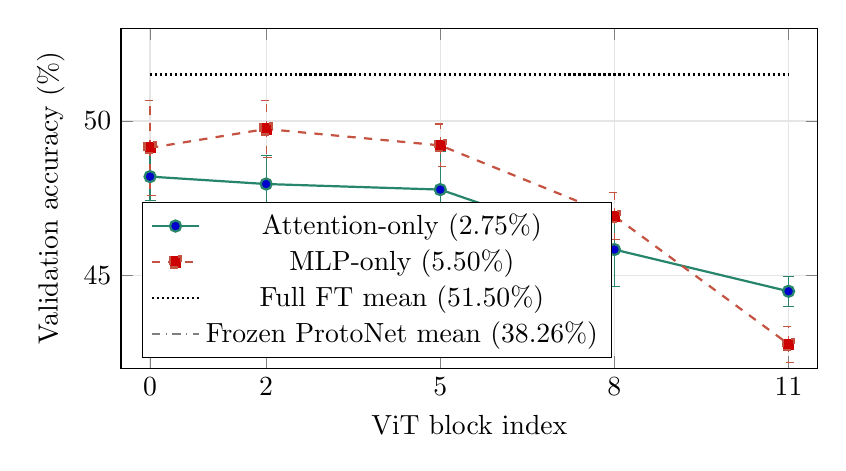
\begin{tikzpicture}
\begin{axis}[
 width=0.86\textwidth,height=5.9cm,
 xlabel={ViT block index},ylabel={Validation accuracy (\%)},
 xtick={0,2,5,8,11},xmin=-0.5,xmax=11.5,ymin=42,ymax=53,
 grid=major,grid style={gray!20},legend pos=south west,
 error bars/y dir=both,error bars/y explicit
]
\addplot+[isiccol,mark=*,thick,error bars/.cd,y dir=both,y explicit] coordinates {
 (0,48.20) +- (0,0.78)
 (2,47.96) +- (0,0.93)
 (5,47.78) +- (0,1.25)
 (8,45.84) +- (0,1.20)
 (11,44.49) +- (0,0.48)
};
\addlegendentry{Attention-only ($2.75\%$)}
\addplot+[mlpcol,mark=square*,thick,dashed,error bars/.cd,y dir=both,y explicit] coordinates {
 (0,49.13) +- (0,1.53)
 (2,49.74) +- (0,0.91)
 (5,49.21) +- (0,0.69)
 (8,46.92) +- (0,0.76)
 (11,42.78) +- (0,0.58)
};
\addlegendentry{MLP-only ($5.50\%$)}
\addplot[black,densely dotted,thick,domain=0:11,samples=2]{51.50};
\addlegendentry{Full FT mean (51.50\%)}
\addplot[gray,dashdotted,thick,domain=0:11,samples=2]{38.26};
\addlegendentry{Frozen ProtoNet mean (38.26\%)}
\end{axis}
\end{tikzpicture}
\caption{ISIC validation depth profiles for both parameter types. Error bars are standard deviations across three episode draws. Each family forms a shallow-to-middle plateau and declines at the deep end. Compare \cref{fig:depthcurves}: the ordering is reversed in both types. No single tested block of either family exceeds the full fine-tuning mean.}
\label{fig:isiccurve}
\end{figure}

The paired comparisons show a consistent reversal of shallow-versus-deep ordering between the datasets, in both measured parameter families. \Cref{tab:mirror} lists six such comparisons; every one is settled on both sides at three draws. This is stronger evidence for dataset-dependent position effects than an isolated comparison of two maxima.

\begin{table}[t]
\centering
\small
\caption{Shallow-versus-deep paired differences, in percentage points, over three episode draws per cell. Every listed comparison takes the opposite sign on the two datasets. Intervals are $\bar{d}\pm t_{0.975,2}s_d/\sqrt{3}$ across draws.}
\label{tab:mirror}
\begin{tabular}{lrr}
\toprule
Shallow $-$ deep & ISIC & EuroSAT\\
\midrule
\multicolumn{3}{l}{\emph{Attention-only} ($2.75\%$ of backbone)}\\
block 2 $-$ block 11 & $+3.47\pm1.14$ & $-7.31\pm1.13$\\
block 5 $-$ block 11 & $+3.28\pm2.07$ & $-4.17\pm1.31$\\
block 5 $-$ block 8 & $+1.93\pm0.23$ & $-5.71\pm1.38$\\
\addlinespace
\multicolumn{3}{l}{\emph{MLP-only} ($5.50\%$ of backbone)}\\
block 0 $-$ block 11 & $+6.35\pm2.37$ & $-4.72\pm2.06$\\
block 2 $-$ block 11 & $+6.96\pm1.16$ & $-4.32\pm0.38$\\
block 2 $-$ block 8 & $+2.82\pm0.41$ & $-8.11\pm0.84$\\
\bottomrule
\end{tabular}
\end{table}

\paragraph{The reversal survives changing the parameter type.} The same five-position sweep was repeated in the block MLP on ISIC: a second family, twice the size, the same depths, the same per-cell learning-rate grid. Mean accuracies across three draws are 49.13\%, 49.74\%, 49.21\%, 46.92\%, and 42.78\% at blocks 0, 2, 5, 8, and 11. The profile has the same shape as the attention curve, and the three MLP rows of \cref{tab:mirror} are settled on both datasets. This separates two readings that the EuroSAT data alone cannot. The reversal could have been something attention does under large shift, in which case it would not appear in the MLP; it appears in the MLP, at a larger margin than in attention ($6.96$ points from block 2 to block 11, against $3.47$). The domain shift rather than the parameter family therefore sets the sign.

One link does \emph{not} reverse, and we state it rather than drop it. Block 5 minus block 11 in the MLP is $+6.43\pm0.63$ on ISIC and $+1.45\pm1.93$ on EuroSAT: the same sign, and unsettled on the EuroSAT side. It is excluded from \cref{tab:mirror} under a criterion we can defend but did not fix before seeing the number, namely that both depths must lie on the same side of the EuroSAT peak as the labels ``shallow'' and ``deep'' claim. Block 11 is \emph{past} the block-8 peak on EuroSAT, so this comparison places two points on the far side of a maximum and is not a shallow-versus-deep contrast at all. The same applies to block 8 minus block 11, which is positive on both datasets ($+4.15\pm0.76$ on ISIC, $+3.80\pm0.97$ on EuroSAT). The fall-off at the final block is the one feature the two curves share.

No single tested block of either family beats full fine-tuning on ISIC. Full fine-tuning averages 51.50\%, compared with 48.20\% for the best attention position (block 0) and 49.74\% for the best MLP position (block 2). The best isolated intervention on EuroSAT therefore should not be generalized into a recommendation for ISIC. The direction of the useful depth shift depends on the target data, and the ISIC plateau does not identify a unique preferred block among blocks 0, 2, and 5.

We use “milder” and “stronger” domain shift as contextual descriptions rather than as a quantitative independent variable. One rough proxy is headroom over the frozen model: the ViT whole-family headroom is 6.34 points for the best family on EuroSAT and 13.24 points for full fine-tuning on ISIC. Those values do not measure domain shift directly and are taken from different best configurations, so they should not be interpreted as a calibrated shift score. The depth curves establish that the preferred positions differ; explaining the difference mechanistically remains future work.

\subsection{Inner-loop length}

\begin{figure}[t]
\centering
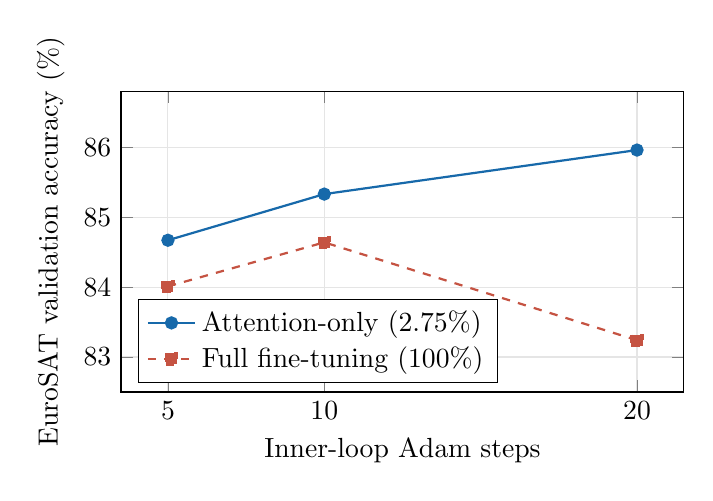
\begin{tikzpicture}
\begin{axis}[
 width=0.72\textwidth,height=5.4cm,
 xlabel={Inner-loop Adam steps},ylabel={EuroSAT validation accuracy (\%)},
 xtick={5,10,20},xmin=3.5,xmax=21.5,ymin=82.5,ymax=86.8,
 grid=major,grid style={gray!20},legend pos=south west,legend cell align=left
]
\addplot[attncol,mark=*,thick] coordinates {
  (5,84.67)
  (10,85.33)
  (20,85.96)
};
\addlegendentry{Attention-only ($2.75\%$)}
\addplot[mlpcol,mark=square*,thick,dashed] coordinates {
  (5,84.01)
  (10,84.64)
  (20,83.24)
};
\addlegendentry{Full fine-tuning ($100\%$)}
\end{axis}
\end{tikzpicture}
\caption{Accuracy against inner-loop length, each baseline retuned at every step
count, one episode draw. Attention-only adaptation improves monotonically with
more updates; full fine-tuning peaks at ten steps and falls by $1.40$ points at
twenty. The $20$-step setting used for the main experiments therefore places
full fine-tuning below its own best step count. Single-draw adjacent differences
are close to the measured run-to-run floor, so this is directional evidence.}
\label{fig:steps}
\end{figure}

\label{sec:steps}

\Cref{fig:steps} shows the result. To test whether the five-shot EuroSAT advantage of attention-only tuning was an artefact of using 20 update steps, we re-tuned both attention-only and full fine-tuning at 5, 10, and 20 steps. \Cref{tab:steps} gives the measured values. At 5 steps the scores were 84.67\% for attention and 84.01\% for full fine-tuning; at 10 steps they were 85.33\% and 84.64\%; at 20 steps they were 85.96\% and 83.24\%. Attention-only performance rose across these settings, while full fine-tuning at 20 steps was 1.40 points below its 10-step result.

\begin{table}[t]
\centering
\small
\caption{EuroSAT validation accuracy under different inner-loop lengths, one episode draw. Each baseline was tuned separately at each step count. These single-draw measurements are directional evidence rather than a replicated test.}
\label{tab:steps}
\begin{tabular}{rrrr}
\toprule
Inner steps & Attention-only (learning rate) & Full FT (learning rate) & Attention $-$ Full\\
\midrule
5 & 84.67\% ($10^{-4}$) & 84.01\% ($3\times10^{-5}$) & +0.65\\
10 & 85.33\% ($10^{-4}$) & 84.64\% ($3\times10^{-5}$) & +0.69\\
20 & 85.96\% ($10^{-4}$) & 83.24\% ($10^{-5}$) & +2.72\\
\bottomrule
\end{tabular}
\end{table}

This is consistent with the possibility that additional optimization harms the large parameter group under scarce support data. However, the 5- and 10-step values are from one draw, and the differences between adjacent step counts are close to the measured run-to-run variation. It would be too strong to conclude that full fine-tuning has a stable optimum at precisely 10 steps. A more defensible conclusion is that the 20-step configuration used in the main experiment places full fine-tuning at a disadvantage relative to its own 10-step validation score, and the direction is consistent with a capacity-versus-data explanation.

\subsection{Support-set size and the bounded advantage}

\begin{figure}[t]
\centering
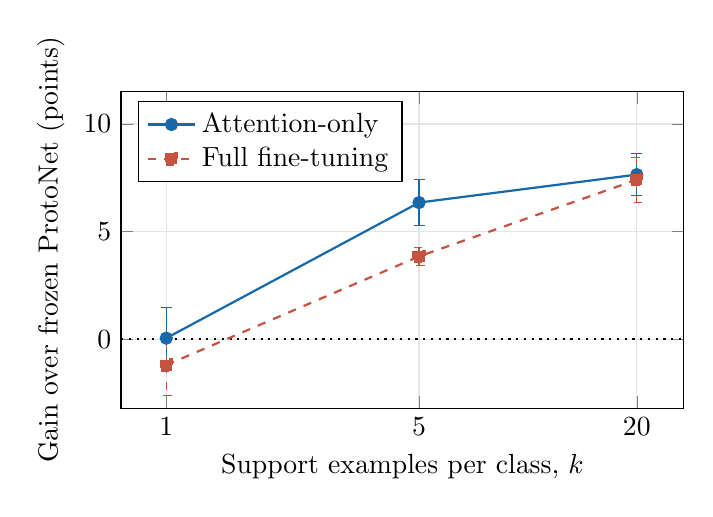
\begin{tikzpicture}
\begin{axis}[
 width=0.72\textwidth,height=5.6cm,
 xmode=log,log basis x=2,
 xlabel={Support examples per class, $k$},
 ylabel={Gain over frozen ProtoNet (points)},
 xtick={1,5,20},xticklabels={1,5,20},xmin=0.75,xmax=27,ymin=-3.2,ymax=11.5,
 grid=major,grid style={gray!20},legend pos=north west,legend cell align=left
]
\addplot[black,dotted,thick,forget plot,domain=0.75:27,samples=2]{0};
\addplot[attncol,mark=*,thick,error bars/.cd,y dir=both,y explicit] coordinates {
  (1,+0.05) +- (0,1.42)
  (5,+6.35) +- (0,1.07)
  (20,+7.65) +- (0,0.98)
};
\addlegendentry{Attention-only}
\addplot[mlpcol,mark=square*,thick,dashed,error bars/.cd,y dir=both,y explicit] coordinates {
  (1,-1.20) +- (0,1.42)
  (5,+3.85) +- (0,0.43)
  (20,+7.41) +- (0,1.04)
};
\addlegendentry{Full fine-tuning}
\end{axis}
\end{tikzpicture}
\caption{Each method's gain over a frozen backbone as support size grows,
EuroSAT. Full fine-tuning is \emph{below} frozen ProtoNet at one shot and has
caught up by twenty; the attention-only advantage is therefore bounded to an
intermediate regime rather than general. The $k=5$ row averages three draws; the
endpoints are single draws, and the statistic was specified after the $k=1$ and
$k=5$ outcomes were seen, so only $k=20$ is a prospective check.}
\label{fig:shots}
\end{figure}

\label{sec:shots}

The support-size probe evaluates $k=1,5,20$ shots per class on EuroSAT; \cref{fig:shots} plots each method's gain over the frozen reference. In the main three-draw five-shot comparison, attention-only reaches 85.56\%, full fine-tuning reaches 83.07\%, and frozen ProtoNet reaches 79.22\%. A separate matched follow-up uses one episode-sampling draw (seed 0) at each support size and compares all three methods on the same episodes. In that paired follow-up, reported in \cref{tab:shots}, attention-only / full fine-tuning / frozen ProtoNet reach 62.15 / 60.89 / 62.09\% at one shot, 85.96 / 83.24 / 79.27\% at five shots, and 94.00 / 93.76 / 86.35\% at twenty shots. The main three-draw five-shot means and the paired seed-0 follow-up are distinct estimates and are not interchanged below.

\begin{table}[t]
\centering
\small
\caption{Matched EuroSAT support-size follow-up on the same episodes within each row (one draw, seed 0). Deltas are paired differences against frozen ProtoNet, in percentage points with episode-level 95\% intervals. The separate three-draw five-shot means are reported in the main parameter-family analysis.}
\label{tab:shots}
\begin{tabularx}{\textwidth}{r r r r Y Y}
\toprule
Shots $k$ & Frozen & Attention & Full FT & Attention $-$ frozen & Full FT $-$ frozen\\
\midrule
1 & 62.09 & 62.15 & 60.89 & $+0.05\pm1.42$ & $-1.20\pm1.42$\\
5 & 79.27 & 85.96 & 83.24 & $+6.69\pm1.21$ & $+3.97\pm1.10$\\
20 & 86.35 & 94.00 & 93.76 & $+7.65\pm0.98$ & $+7.41\pm1.04$\\
\bottomrule
\end{tabularx}
\end{table}

The attention-minus-full-fine-tuning gap is $+1.25\pm1.18$ points at one shot, $+2.50\pm0.64$ in the three-draw five-shot benchmark, and $+0.24\pm0.53$ at twenty shots. The gap alone is not a clean test of over-optimization: at one shot, neither adapted method improves materially over frozen ProtoNet, while at twenty shots the full model has caught up. In the matched seed-0 follow-up, full fine-tuning's gain over frozen rises from $-1.20$ points at one shot to $+3.97$ at five shots and $+7.41$ at twenty shots; attention-only's corresponding gains are $+0.05$, $+6.69$, and $+7.65$. The twenty-shot frozen result (86.35\%) shows that both models still benefit substantially from adaptation, so the closed gap is not simply caused by frozen and adapted accuracies all saturating together.

There is an important inferential qualification: the gain-over-frozen statistic was formulated after the one- and five-shot outcomes had been inspected. The twenty-shot row was the prospective check of that revised prediction, not a preregistered test of the original hypothesis. Furthermore, the follow-up uses one draw at each support size, and the one-shot differences against frozen include zero within their 95\% intervals. The pattern is consistent with full fine-tuning benefiting more as support data increases, but it is limited evidence for a capacity-versus-data explanation rather than a conclusive mechanism test.

\subsection{Weight decay: the predicted repair fails}

\begin{figure}[t]
\centering
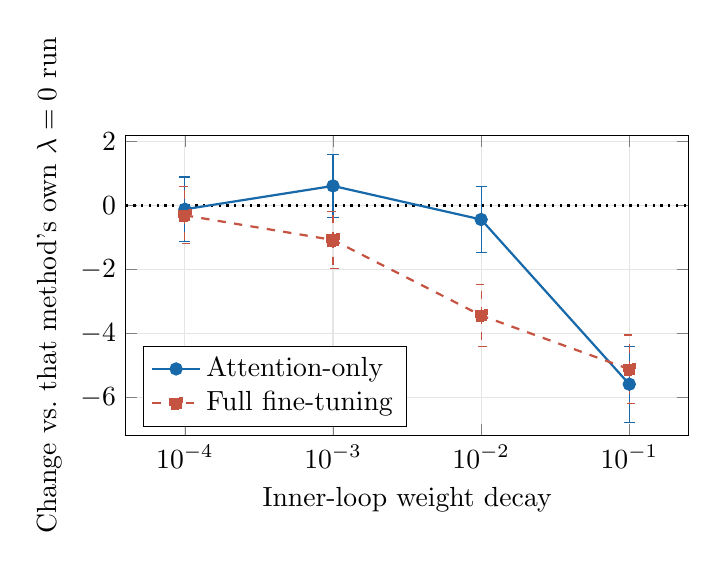
\begin{tikzpicture}
\begin{axis}[
 width=0.72\textwidth,height=5.4cm,
 xlabel={Inner-loop weight decay},
 ylabel={Change vs.\ that method's own $\lambda=0$ run},
 xtick={1,2,3,4},xticklabels={$10^{-4}$,$10^{-3}$,$10^{-2}$,$10^{-1}$},
 xmin=0.6,xmax=4.4,ymin=-7.2,ymax=2.2,
 grid=major,grid style={gray!20},legend pos=south west,legend cell align=left
]
\addplot[black,dotted,thick,forget plot,domain=0.6:4.4,samples=2]{0};
\addplot[attncol,mark=*,thick,error bars/.cd,y dir=both,y explicit] coordinates {
  (1,-0.12) +- (0,1.01)
  (2,+0.61) +- (0,0.99)
  (3,-0.44) +- (0,1.03)
  (4,-5.59) +- (0,1.19)
};
\addlegendentry{Attention-only}
\addplot[mlpcol,mark=square*,thick,dashed,error bars/.cd,y dir=both,y explicit] coordinates {
  (1,-0.31) +- (0,0.89)
  (2,-1.08) +- (0,0.89)
  (3,-3.44) +- (0,0.98)
  (4,-5.12) +- (0,1.07)
};
\addlegendentry{Full fine-tuning}
\end{axis}
\end{tikzpicture}
\caption{The predicted repair fails. If full fine-tuning lost because too many
parameters moved too freely, regularisation should have recovered it. Instead the
dose response is monotonically negative, reaching $-5.12$ points at
$\lambda=10^{-1}$. Attention-only adaptation is flat until $10^{-2}$ and is
then damaged as well, so a small parameter group is not inherently immune.
Differences are paired against each method's own $\lambda=0$ run on the same
episodes; the two arms use separately tuned learning rates, so only the
within-method dose response is clean.}
\label{fig:wd}
\end{figure}

\label{sec:wd}

\Cref{fig:wd} plots the dose response. The capacity-versus-data account motivated a direct intervention: if full fine-tuning suffers because too many parameters move too far from a useful pretrained representation, regularization might constrain its updates. In the executed experiment, increasing coupled Adam weight decay did not repair full fine-tuning. Relative to the corresponding zero-decay configuration (\cref{tab:wd}), the paired changes in EuroSAT accuracy were $-0.31\pm0.89$ at $10^{-4}$, $-1.08\pm0.89$ at $10^{-3}$, $-3.44\pm0.98$ at $10^{-2}$, and $-5.12\pm1.07$ at $10^{-1}$. The decline is monotonic and becomes clearly detrimental at the larger tested values.

\begin{table}[t]
\centering
\small
\caption{Paired changes in EuroSAT validation accuracy relative to each method's own zero-decay run (one episode draw). Entries are percentage-point differences with episode-paired 95\% intervals.}
\label{tab:wd}
\begin{tabular}{lrrrrr}
\toprule
Method & $\lambda=0$ accuracy & $10^{-4}$ & $10^{-3}$ & $10^{-2}$ & $10^{-1}$\\
\midrule
Full FT & 83.56\% & $-0.31\pm0.89$ & $-1.08\pm0.89$ & $-3.44\pm0.98$ & $-5.12\pm1.07$\\
Attention-only & 85.36\% & $-0.12\pm1.01$ & $+0.61\pm0.99$ & $-0.44\pm1.03$ & $-5.59\pm1.19$\\
\bottomrule
\end{tabular}
\end{table}

The prediction that weight decay would rescue full fine-tuning fails. The result should not be silently reinterpreted as a successful regularization test. One plausible explanation is that conventional weight decay pulls parameters toward zero rather than toward their pretrained values. That distinction is important in transfer learning: “remain close to the initialization” is better expressed by a penalty on $\|\theta-\theta_0\|^2$ than by a penalty on $\|\theta\|^2$. But the explanation is post hoc and the corresponding $\ell^2$-SP experiment was not run. It remains a hypothesis, not an established mechanism.

There is also an across-baseline confound. The optimiser uses coupled L2 with Adam rather than decoupled AdamW, and full fine-tuning and attention-only adaptation use learning rates differing by an order of magnitude. Equal nominal decay values therefore do not imply equal effective regularization strength across the methods. The within-full-fine-tuning dose response is the cleanest comparison because only the decay level varies. Attention-only adaptation is also strongly damaged at $10^{-1}$, so the results do not support a claim that a small parameter group is inherently immune to regularization.

\section{Discussion}
\label{sec:discussion}

\subsection{What the depth curves establish}

The clearest result is not simply that partial tuning can beat full fine-tuning. That observation already appears in PEFT and partial fine-tuning literature \cite{basu2024,lian2022,ye2023}. The stronger point is that, for a fixed parameter family within the evaluated ViT-B/16, the position of the trainable block is associated with a large performance difference. Attention-only adaptation ranges over 8.85 points on EuroSAT across the five sampled depths, while MLP-only adaptation ranges over 8.52 points. Both peak at block 8; shallow attention blocks offer little gain over the frozen model. Since each selected block has the same nominal parameter count within a family, the curve cannot be explained merely by “more parameters were updated at the good depth.”

The ISIC profile gives the result its key qualification, and it holds in both measured families. The shallow-to-middle region is best on this dataset for attention and MLP alike, and deep interventions are weaker. Moreover, no single tested block of either family beats full fine-tuning. Thus, the correct inference is that depth is a consequential, dataset-dependent variable, not that one depth is universally optimal or that partial adaptation should always replace full fine-tuning. The fact that the curve reverses in sign between target datasets is a reason for further controlled experiments, not enough evidence to fit a general law of depth and domain-shift magnitude.

\subsection{Why whole-family averages can be misleading}

A whole-network attention-only run updates attention projections throughout all twelve blocks. A single-block run changes one location. The whole-family comparison therefore averages together blocks with distinct measured outcomes. In EuroSAT, attention-only full-family tuning scores 85.56\% across three draws, below the 87.49\% mean for attention in block 8 alone. The MLP-only family similarly averages across its shallow, middle, and deep positions, while MLP block 8 yields 88.79\%. A conclusion about the performance of “attention-only tuning” or “MLP-only tuning” can consequently depend on the depth distribution implied by the selector.

This interpretation does not show that whole-network parameter-family comparisons are useless. They answer a practical question about a specific strategy that updates an entire family. They do not answer the separate question about the best possible member of that family if its position is allowed to vary. The two axes should be evaluated separately and, where interactions are plausible, jointly.

\subsection{What the ResNet pilot contributed}

The ResNet pilot was not discarded simply because the gate failed. It established an important research-design constraint. A controller can only improve adaptation if its signals encode information relevant to which updates help, and the tested utility/drift signals did not provide that information reliably. Moreover, the gate as implemented did not achieve sparse adaptation. Moving directly to a more elaborate controller would have mixed an unproven signal model with a more complex optimizer.

The ViT study removes the controller and tests placement by intervention. This pivot also improves the experimental control: ViT blocks are structurally matched, while ResNet stages vary substantially in size and resolution. The resulting paper is therefore not a demonstration that the originally proposed full ARC controller works. It is an empirical investigation whose motivating controller did not produce the expected benefit and whose follow-up analysis isolates a clearer phenomenon.

\subsection{The mechanism remains incomplete}

The inner-step results are consistent with the idea that full fine-tuning is more sensitive to optimization length under few-shot supervision. The matched support-size follow-up adds a complementary pattern: full fine-tuning is numerically below frozen ProtoNet at one shot, then gains about 3.97 points over frozen at five shots and 7.41 points at twenty shots. At twenty shots, both adaptation methods still gain substantially over frozen ProtoNet, while their difference is near zero. However, the support-size statistic was revised after seeing the lower-shot results, only the twenty-shot row was prospective relative to that revised statistic, and the endpoint measurements are single draws. Weight decay, intended as a direct regularization intervention, harms full fine-tuning rather than improving it. Taken together, the evidence is consistent with a capacity-sensitive account but does not establish a complete causal mechanism.

The paper therefore separates the empirical depth result from the proposed explanation. The depth result is supported by repeated paired depth curves. The explanation remains provisional and should be tested through more support sizes, more episode draws, regularization toward the pretrained initialization, and direct measures of how parameter updates relate to the target task. Keeping those claims separate protects the main finding from depending on a mechanism test that did not succeed.

\subsection{Implications for adaptation design}

The results suggest three practical guidelines for evaluating adaptation methods under few-shot domain shift.
\begin{enumerate}
  \item \textbf{Do not infer a best location from parameter count alone.} Equal-sized parameter groups can produce very different outcomes depending on where they are placed.
  \item \textbf{Tune groups individually, and document the tuning process.} Learning-rate optima can differ by orders of magnitude between small and large parameter groups. A comparison at one shared learning rate risks measuring hyperparameter mismatch instead of the method.
  \item \textbf{Do not promote a dataset-specific winner into a universal prescription.} EuroSAT and ISIC show different depth profiles. A deployment setting should validate selection on data that represents its domain, with a held-out evaluation that was not used to choose the position.
\end{enumerate}

The study does not establish that a simple depth sweep is the most compute-efficient procedure in every application. It does show why adaptive layer selectors should be evaluated against a controlled fixed-depth baseline and why parameter family and layer position are distinct design variables.

\section{Limitations and threats to validity}
\label{sec:limitations}

\paragraph{Validation-only results.} The train/validation/test partitions are fixed, but the reported headline results all come from validation. The test partition was deliberately held out while the study's design choices were still changing. This is preferable to tuning against the test set, but it means the manuscript does not establish test-set generalization. A final test evaluation must be conducted only after the protocol, selected comparisons, and hyperparameters are frozen.

\paragraph{Two target datasets.} EuroSAT and ISIC differ in domain and difficulty, and their depth profiles differ. Two datasets are not enough to infer a general function from domain shift to optimal adaptation depth. Headroom over frozen ProtoNet is only a proxy for adaptation opportunity and should not be mistaken for a direct measure of distribution shift.

\paragraph{Two parameter families.} Both attention-only and MLP-only adaptation are now measured at all five sampled depths on both datasets, so the dataset-dependent reversal is not a single-family finding. The backbone nevertheless admits other families -- LayerNorm, patch embedding, and combinations across families -- which are measured only at whole-network scope, not across depth. The depth sweep therefore covers two of the parameter families this paper partitions, not all of them.

\paragraph{Only five of twelve depths.} The sweeps measure blocks 0, 2, 5, 8, and 11. The observed interior peak on EuroSAT lies at block 8 among the tested locations; the experiment does not show that block 8 is the best of all twelve blocks. A denser sweep around blocks 6--10 is required to localize the peak more precisely.

\paragraph{One architecture family.} The main depth finding is measured with a ViT-B/16 initialized from supervised ImageNet-21k pretraining. It is not established for other ViT sizes, self-supervised pretraining, ConvNets, or other vision architectures. The ResNet-50 pilot is not a matched replication of the ViT depth intervention because ResNet units do not provide the same uniform block structure.

\paragraph{Unequal replication across secondary probes.} The primary depth profiles use three episode-sampling seeds, each with 100 episodes. The parameter-family table includes some single-draw cells. Inner-step and weight-decay studies are single-draw probes; shot-size results at $k=1$ and $k=20$ are also single draws. These are reported as directional or descriptive evidence rather than equally strong confirmation of the main finding.

\paragraph{Hyperparameter-selection effects.} Learning rates were selected using the validation split and the main comparisons reflect these choices. Using independently tuned settings is necessary because groups have different optimization scales, but it also means the comparison is between tuned strategies, not under a shared learning rate. Multiple choices were examined during development, and no held-out test result is available to estimate remaining selection optimism.

\paragraph{Run-to-run optimization nondeterminism.} Fine-tuning runs show a practical variation floor near 0.6 points for repeated settings. The paired use of common episodes reduces episode-difficulty variance, and three draws improve the reliability of main depth comparisons. It does not eliminate every source of GPU nondeterminism or the uncertainty induced by only three draws.

\paragraph{No direct common-protocol comparison against external PEFT methods.} Published SSF, LN-Tune, DIPA, ALaST, and LoRA results use different data, backbones, pretraining objectives, or tasks. We compare their methodological motivations, not their reported accuracies. A head-to-head study with consistent checkpoints and protocol is needed before claiming the proposed depth-selective strategy is superior to any external method.

\paragraph{Mechanism not proved.} The inner-step probe and a matched support-size follow-up are consistent with full fine-tuning becoming more useful as support data grows. However, the revised gain-over-frozen prediction was formulated after examining the one- and five-shot outcomes, with the twenty-shot row serving as the prospective check; the endpoint measurements are single draws and the probe is EuroSAT-only. The weight-decay intervention fails in the predicted direction, and an initialization-centred penalty such as $\ell^2$-SP has not been run. These findings therefore do not establish the cause of the depth-dependent outcomes.

\paragraph{No forensic-domain validation in the current benchmark.} The initial project framing involved forensic trace evidence. The experiments reported here instead use public image-classification datasets because the intended forensic data sources were not available in a verified, reproducible form for this evaluation. The findings are methodological results about cross-domain few-shot vision, not a claim of validated performance on forensic evidence.

\section{Conclusion}

This paper studies adaptation depth as a distinct choice from parameter family in cross-domain few-shot vision. In a ViT-B/16, adapting the same parameter family in different blocks leads to materially different validation accuracy. On EuroSAT, the attention-only curve has a strong interior peak at block 8, and a parallel MLP-only curve exhibits a comparable peak. On ISIC, shallow-to-middle blocks are stronger than deeper positions and no single tested block beats full fine-tuning. These observations establish a dataset-dependent depth effect under the evaluated protocol, rather than a universal rule for where to adapt.

The work also documents the research trajectory that motivated the controlled study. A ResNet-50 adaptive gate based on utility and drift did not produce a reliable gain, and the follow-up diagnostics did not support extending that controller without a better account of which adaptation signals predict useful updates. The ViT experiments provide a cleaner, more direct measurement of depth. Inner-step and support-size probes are consistent with full fine-tuning benefiting increasingly from more support data, but the support-size statistic was revised after lower-shot outcomes were observed and the weight-decay intervention fails. The mechanism therefore remains provisional rather than established.

The main implication is methodological: adaptation depth should be measured, not assumed to be irrelevant once parameter family and trainable parameter count are fixed. Future work should expand the depth sweep, test more target domains and backbones, report held-out test results, and compare depth-selective updates directly against strong PEFT baselines under a common protocol. The present results are validation evidence that placement matters; they are not yet a general prescription for every few-shot transfer task.

\appendix
\section{Parameter counts and adaptation configurations}

\begin{table}[!htbp]
\centering
\small
\caption{Parameter-family partition for ViT-B/16 used in the main experiments. Counts are those asserted by the selector implementation.}
\label{tab:paramcounts}
\begin{tabularx}{\textwidth}{lrrY}
\toprule
Configuration & Parameters & Fraction & Interpretation\\
\midrule
Frozen ProtoNet & 0 trainable backbone parameters & 0\% & Backbone frozen; only episode prototypes are formed from the support set.\\
LayerNorm scale & 19,200 & 0.022\% & Update LayerNorm scale parameters only.\\
LayerNorm shift & 19,200 & 0.022\% & Update LayerNorm bias parameters only.\\
LayerNorm only & 38,400 & 0.045\% & Update scale and shift parameters across the network.\\
Patch embedding & 742,656 & 0.866\% & Update the image patch projection/embedding parameters.\\
Attention only & 28,348,416 & 33.041\% & Update attention projections across all twelve blocks.\\
MLP only & 56,669,184 & 66.049\% & Update feed-forward MLP parameters across all twelve blocks.\\
Full fine-tuning & 85,798,656 & 100\% & Update all parameters covered by the experiment's selector partition.\\
Single attention block & Approx. 2.36M & Approx. 2.75\% & Update attention projections in one selected block only.\\
Single MLP block & Approx. 4.72M & Approx. 5.50\% & Update MLP parameters in one selected block only.\\
\bottomrule
\end{tabularx}
\end{table}

\section{Additional results from the ResNet-50 pilot}

\subsection{ISIC tuned baseline comparison}

\begin{table}[!htbp]
\centering
\small
\caption{ResNet-50 ISIC validation baseline measurements at five shots. Values are single configuration summary values from the pilot baseline runs.}
\label{tab:isicresnet}
\begin{tabular}{lrr}
\toprule
Method & Learning rate & Accuracy (\%)\\
\midrule
Full fine-tuning & $10^{-4}$ & 49.55\\
BatchNorm-only fine-tuning & $3\times10^{-2}$ & 49.44\\
Progressive unfreezing & $10^{-4}$ & 47.15\\
Stage-4 fine-tuning & $3\times10^{-4}$ & 46.52\\
Last-layer fine-tuning & $3\times10^{-3}$ & 43.64\\
\bottomrule
\end{tabular}
\end{table}

\Cref{tab:isicresnet} lists the ISIC pilot baselines. The near-equality between BatchNorm-only tuning and full fine-tuning is restricted to this validation protocol and these individually selected learning rates. It does not imply that normalisation tuning is always sufficient on medical imagery, nor that BatchNorm and LayerNorm experiments are interchangeable.

\subsection{Activation-space displacement probe}

The ResNet subspace diagnostic decomposed the measured per-channel activation displacement into shift, scale, and residual components on a probe batch. For the ISIC measurements in the experiment log, a per-channel affine account captured approximately 90\% of the full-fine-tuning displacement and approximately 95\% of the BatchNorm-only displacement. These percentages describe the measured activations and probe construction, not universal function approximation error. A low-dimensional or diagonal activation displacement does not guarantee that a correction learned from one set of support/query activations will generalize across different episodes.

The offline correction experiments also found that the estimate depends on the adaptation runs used to extract it. Two nominally identical extraction runs produced a roughly two-point spread in downstream validation accuracy. Accordingly, any precomputed correction result should be reported with extraction-run variance as well as episode-sampling variance. This paper does not promote the offline correction into a main method or use its best single extraction score as evidence that zero-step adaptation replaces fine-tuning.

\section{Reproducibility checklist}

\begin{table}[!htbp]
\centering
\small
\caption{Protocol elements relevant to reproducing the main ViT results.}
\label{tab:repro}
\begin{tabularx}{\textwidth}{P{0.28\textwidth}Y}
\toprule
Element & Specification\\
\midrule
Backbone & ViT-B/16, supervised ImageNet-21k AugReg checkpoint \method{vit\_base\_patch16\_224.augreg\_in21k}.\\
Datasets & EuroSAT and ISIC 2018 / HAM10000.\\
Input resolution & 224 by 224 pixels, using the experiment's standard checkpoint-compatible transform.\\
Episode & 5-way classification, 5 labelled support examples per class, 15 query examples per class for the main experiment.\\
Main depth positions & Blocks 0, 2, 5, 8, 11; attention-only and MLP-only sublayer selectors.\\
Main inner-loop length & 20 Adam steps on the support objective.\\
Hyperparameter selection & Learning-rate grid tuned on validation; selected values fixed for additional episode seeds in the headline curves.\\
Sampling & 100 episodes per draw for main depth curves; episode seeds 0, 1, 2; split seed 0.\\
Primary metrics & Mean episode accuracy, standard deviation across draws, and paired per-seed accuracy differences.\\
ISIC leakage control & Group-disjoint split by lesion identifier from HAM10000 metadata.\\
Test-set status & Test split held out; no held-out test results are reported in this manuscript.\\
Unresolved mechanisms & Initialization-centred $\ell^2$-SP, denser depth scan, additional backbones/datasets, and external PEFT reruns remain future work.\\
\bottomrule
\end{tabularx}
\end{table}

\section{Scope of claims}

\Cref{tab:paramcounts} gives the exact parameter partition and \cref{tab:repro} the protocol elements needed to reproduce the main results. For clarity, the paper makes the following distinctions:
\begin{itemize}
  \item The reported 8.85-point attention span and 8.52-point MLP span are validation differences among five sampled depths on EuroSAT, averaged over three episode draws.
  \item The claim that the preferred depth profile changes by dataset is supported by six paired shallow/deep comparisons over three draws on EuroSAT and ISIC, three in attention-only adaptation and three in MLP-only adaptation. Two further MLP comparisons involving block 11 do not reverse; they are excluded from \cref{tab:mirror} because block 11 lies past the EuroSAT peak, and that exclusion criterion was chosen after the numbers were seen rather than in advance.
  \item The claim that attention-only and MLP-only adaptation each have an interior peak refers to the tested positions; it is not a claim that block 8 is the global optimum across all twelve blocks.
  \item The capacity-versus-data account is a provisional interpretation supported by a single-draw inner-step probe and a matched support-size follow-up. The gain-over-frozen statistic was revised after inspecting lower-shot outcomes; only the twenty-shot row was prospective relative to that revised prediction. Weight decay does not rescue full fine-tuning, so the mechanism remains unproven.
  \item The original multi-signal ARC controller, topological signal, stability signal, novelty signal, and FBSDE controller are not presented as completed experiments.
  \item No published baseline accuracy is presented as a direct head-to-head comparison unless it was rerun under the same data, backbone, pretraining, and episodic protocol. No such external comparator is included here.
\end{itemize}

\begin{thebibliography}{99}

\bibitem{basu2024}
S. Basu, S. X. Hu, D. Massiceti, and S. Feizi.
\newblock Strong baselines for parameter-efficient few-shot fine-tuning.
\newblock In \emph{Proceedings of the AAAI Conference on Artificial Intelligence}, 38(10):11024--11031, 2024.
\newblock doi:10.1609/aaai.v38i10.28978.

\bibitem{codella2019}
N. Codella, V. Rotemberg, P. Tschandl, M. E. Celebi, S. Dusza, D. Gutman, B. Helba, A. Kalloo, K. Liopyris, M. Marchetti, J. K. Kittler, and others.
\newblock Skin lesion analysis toward melanoma detection 2018: A challenge hosted by the International Skin Imaging Collaboration (ISIC).
\newblock \emph{arXiv preprint arXiv:1902.03368}, 2019.

\bibitem{devoto2025}
A. Devoto, F. Alvetreti, J. Pomponi, P. Di Lorenzo, P. Minervini, and S. Scardapane.
\newblock Adaptive layer and token selection for efficient fine-tuning of vision transformers.
\newblock \emph{Neurocomputing}, 654:131216, 2025.
\newblock doi:10.1016/j.neucom.2025.131216.

\bibitem{guo2020}
Y. Guo, N. C. Codella, L. Karlinsky, J. V. Codella, J. R. Smith, K. Saenko, T. Rosing, and R. Feris.
\newblock A broader study of cross-domain few-shot learning.
\newblock In \emph{Proceedings of the European Conference on Computer Vision (ECCV)}, 2020.

\bibitem{helber2019}
P. Helber, B. Bischke, A. Dengel, and D. Borth.
\newblock EuroSAT: A novel dataset and deep learning benchmark for land use and land cover classification.
\newblock \emph{IEEE Journal of Selected Topics in Applied Earth Observations and Remote Sensing}, 12(7):2217--2226, 2019.

\bibitem{lian2022}
D. Lian, D. Zhou, J. Feng, and X. Wang.
\newblock Scaling and shifting your features: A new baseline for efficient model tuning.
\newblock In \emph{Advances in Neural Information Processing Systems}, 35, 2022.

\bibitem{lora2022}
E. J. Hu, Y. Shen, P. Wallis, Z. Allen-Zhu, Y. Li, S. Wang, L. Wang, and W. Chen.
\newblock LoRA: Low-rank adaptation of large language models.
\newblock In \emph{International Conference on Learning Representations (ICLR)}, 2022.

\bibitem{nakamura2019}
A. Nakamura and T. Harada.
\newblock Revisiting fine-tuning for few-shot learning.
\newblock \emph{arXiv preprint arXiv:1910.00216}, 2019.

\bibitem{nie2024}
J. Nie, Y. Xing, G. Zhang, Y. Yan, A. Xiao, Y.-P. Tan, A. Kot, and S. Lu.
\newblock Cross-domain few-shot segmentation via iterative support-query correspondence mining.
\newblock In \emph{Proceedings of the IEEE/CVF Conference on Computer Vision and Pattern Recognition (CVPR)}, pages 3380--3390, 2024.

\bibitem{perera2024}
R. Perera and S. Halgamuge.
\newblock Discriminative sample-guided and parameter-efficient feature space adaptation for cross-domain few-shot learning.
\newblock In \emph{Proceedings of the IEEE/CVF Conference on Computer Vision and Pattern Recognition (CVPR)}, pages 23794--23804, 2024.

\bibitem{snell2017}
J. Snell, K. Swersky, and R. Zemel.
\newblock Prototypical networks for few-shot learning.
\newblock In \emph{Advances in Neural Information Processing Systems}, 30, 2017.

\bibitem{steiner2022}
A. Steiner, A. Kolesnikov, X. Zhai, R. Wightman, J. Uszkoreit, and L. Beyer.
\newblock How to train your ViT? Data, augmentation, and regularization in vision transformers.
\newblock \emph{Transactions on Machine Learning Research}, 2022.

\bibitem{tschandl2018}
P. Tschandl, C. Rosendahl, and H. Kittler.
\newblock The HAM10000 dataset, a large collection of multi-source dermatoscopic images of common pigmented skin lesions.
\newblock \emph{Scientific Data}, 5:180161, 2018.
\newblock doi:10.1038/sdata.2018.161.

\bibitem{vit2021}
A. Dosovitskiy, L. Beyer, A. Kolesnikov, D. Weissenborn, X. Zhai, T. Unterthiner, M. Dehghani, M. Minderer, G. Heigold, S. Gelly, J. Uszkoreit, and N. Houlsby.
\newblock An image is worth 16$\times$16 words: Transformers for image recognition at scale.
\newblock In \emph{International Conference on Learning Representations (ICLR)}, 2021.

\bibitem{yang2023}
B. Yang, M. Lin, Y. Zhang, B. Liu, X. Liang, R. Ji, and Q. Ye.
\newblock Dynamic support network for few-shot class-incremental learning.
\newblock \emph{IEEE Transactions on Pattern Analysis and Machine Intelligence}, 45(3):2945--2951, 2023.
\newblock doi:10.1109/TPAMI.2022.3175849.

\bibitem{ye2023}
P. Ye, Y. Huang, C. Tu, M. Li, T. Chen, T. He, and W. Ouyang.
\newblock Partial fine-tuning: A successor to full fine-tuning for vision transformers.
\newblock \emph{arXiv preprint arXiv:2312.15681}, 2023.

\bibitem{zhuang2025}
X. Zhuang, G. Peeters, and G. Richard.
\newblock Episode-specific fine-tuning for metric-based few-shot learners with optimization-based training.
\newblock \emph{arXiv preprint arXiv:2506.17499}, 2025.

\end{thebibliography}

\end{document}
